%\documentclass[landscape]{foils}
\documentclass[25pt,landscape]{foils}

\usepackage{color,amsmath}
\usepackage{amssymb}
\usepackage{amsmath}
\usepackage{booktabs}
\usepackage{hyperref}
\usepackage[thicklines]{cancel}
\usepackage[absolute]{textpos}
\textblockorigin{-1mm}{-1mm}

\newif\ifpdf
\ifx\pdfoutput\undefined
  \pdffalse                     % we are not running pdflatex
  \usepackage[dvips]{graphicx}
\else
  \pdfoutput=1                  % we are running pdflatex
  \pdftrue
  \pdfcompresslevel9
  \usepackage[pdftex]{graphicx}
\fi

%%%%%%%%%%%%%%%%%%%%%%%%%%%%%%%%%%%%%%%%%%%%%%%%%%%%%%%%%%%%%%%%%%%%%%

\definecolor{mypine}{rgb}{0.05,0.45,0.05}
\definecolor{mypurple}{rgb}{0.75,0.0,0.75}
\definecolor{mygray}{rgb}{0.35,0.35,0.35}
\definecolor{niceblue}{rgb}{0.25,0.25,1}
\definecolor{mylightgray}{rgb}{0.5,0.5,0.5}
\newcommand{\Red}{\textcolor{red}}
\newcommand{\Blue}{\textcolor{blue}}
\newcommand{\Niceblue}{\textcolor{niceblue}}
\newcommand{\Gray}{\textcolor{mygray}}
\newcommand{\LightGray}{\textcolor{mylightgray}}
\newcommand{\Purple}{\textcolor{mypurple}}
\newcommand{\Green}{\textcolor{mypine}}
\newcommand{\Cyan}{\textcolor{cyan}}
\newcommand{\PineGreen}{\textcolor{mypine}}
\newcommand{\DarkGreen}{\textcolor{mypine}}

% mathclap
\def\clap#1{\hbox to 0pt{\hss#1\hss}}
\def\mathllap{\mathpalette\mathllapinternal}
\def\mathrlap{\mathpalette\mathrlapinternal}
\def\mathclap{\mathpalette\mathclapinternal}
\def\mathllapinternal#1#2{%
\llap{$\mathsurround=0pt#1{#2}$}}
\def\mathrlapinternal#1#2{%
\rlap{$\mathsurround=0pt#1{#2}$}}
\def\mathclapinternal#1#2{%
\clap{$\mathsurround=0pt#1{#2}$}}

\newcommand{\myfoilhead}[1]{
\newpage
\vspace*{-1cm}
\Gray{
\begin{tabular*}{\textwidth}{l}
{\bf \Huge #1} \\
\bottomrule
\end{tabular*}}}

\newcommand{\mymessage}[2]{
\newpage
\vspace*{-1cm}
%\LightGray{
%{\Huge \tt \textless messages\textgreater}}
\vfill
\begin{tabular*}{\textwidth}{l}
%\toprule
{\bf \Huge #1} \\[0.3in]
%\midrule
\hspace*{0.1\linewidth}\begin{minipage}{0.89\linewidth}
    \Large #2
\end{minipage}\\
%\bottomrule
\end{tabular*}
\vfill
%\LightGray{{\Huge \hspace*\textwidth\llap{\tt \textless/messages\textgreater}}}
}

\newcommand{\myindent}[1]{
\hspace*{0.1\linewidth}\begin{minipage}{0.89\linewidth}
    #1
\end{minipage}}


% A4 = 210 mm x 297 mm
\parindent=0em
\parskip=0em
% \textheight=191mm
\textheight=7.5in
\oddsidemargin=-0.5in
% \textwidth=275mm
\textwidth=10in
\topmargin=-0.7in
\pagestyle{empty}

%\newcommand{\ave}[2]{\left< #2 \right>_{#1}}
\newcommand{\ave}[2]{{\mathbb E}_{#1}\kern-2pt\left[ #2 \right]}
%\newcommand{\var}[2]{{\mathrm{var}}_{#1}\left[ #2 \right]}
\newcommand{\var}[2]{{\mathrm{var}}_{#1}\kern-2pt\left[ #2 \right]}

\newcommand{\sth}{^{(s)}}
\newcommand{\I}{\mathbb I}
\newcommand{\bh}{\mathbf{h}}
\newcommand{\bx}{\mathbf{x}}
\newcommand{\bz}{\mathbf{z}}
\newcommand{\bu}{\mathbf{u}}
\newcommand{\D}{\mathcal{D}}
\newcommand{\M}{\mathcal{M}}
\newcommand{\N}{\mathcal{N}}
\newcommand{\Z}{\mathcal{Z}}
\newcommand{\la}{\!\leftarrow\!}
\newcommand{\ra}{\!\rightarrow\!}
\newcommand{\te}{\!=\!}
\newcommand{\myvcenter}[1]{\ensuremath{\vcenter{\hbox{#1}}}} % vertical centering

\newcommand{\g}{\!\mid\!} % ``given''

%%%%%%%%%%%%%%%%%%%%%%%%%%%%%%%%%%%%%%%%%%%%%%%%%%%%%%%%%%%%%%%%%%%%%%
%%%%%%%%%%%%%%%%%%%%%%%%%%%%%%%%%%%%%%%%%%%%%%%%%%%%%%%%%%%%%%%%%%%%%%
\begin{document}

\myfoilhead{Markov chain Monte Carlo}

\bigskip

\begin{flushright}
{Machine Learning Summer School 2009}

{\texttt{http://mlg.eng.cam.ac.uk/mlss09/}}
\bf Iain Murray}\\
%\texttt{murray@cs.toronto.edu}
\texttt{http://www.cs.toronto.edu/\~{}murray/
\end{flushright}

\vspace*{5cm}

%\Red{\textbf{Draft slides\\Subject to change}}
~\\
~

\vspace*{-5cm}

\begin{flushright}
    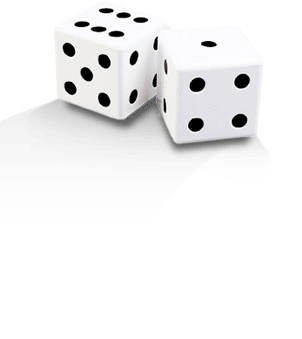
\includegraphics[scale=1.1]{dice}
\end{flushright}

\vfill
\vspace*{-10cm}
{\bf Iain Murray}\\
%\texttt{murray@cs.toronto.edu}
\texttt{http://www.cs.toronto.edu/\~{}murray/}

%%%%%%%%%%%%%%%%%%%%%%%%%%%%%%%%%%%%%%%%%%%%%%%%%%%%%%%%%%%%%%%%%%%%%%
\myfoilhead{A statistical problem}

\vfill

\textbf{What is the average height of the MLSS lecturers?}\\
Method: measure their heights, add them up and divide by $N\te20$.

\vfill

\textbf{What is the average height $f$ of people $p$ in Cambridge ${\mathcal C}$?}\\
\[
\begin{split}
E_{p\in \mathcal C}[f(p)] &\equiv 
\frac{1}{|{\mathcal C}|} \sum_{p\in \mathcal C} f(p),~~\mbox{``intractable''?} \\[0.2in]
&\approx \frac{1}{S} \sum_{s=1}^{S} f\big(p^{(s)}\big),~~
\mbox{for random survey of $S$ people $\{p^{(s)}\}\in{\mathcal C}$}
\end{split}
\]

\vfill
\Green{Surveying works for large and notionally infinite populations.}
%Good answers available with modest sample sizes,\\
%even if the population is large or notionally infinite

%%%%%%%%%%%%%%%%%%%%%%%%%%%%%%%%%%%%%%%%%%%%%%%%%%%%%%%%%%%%%%%%%%%%%%
\myfoilhead{Simple Monte Carlo}

\vfill

Statistical sampling can be applied to any expectation:

\vfill

\Green{\bf In general:}\\[-0.2in]
\[
\Blue{\int} f(x) \Blue{P(x) \;\mathrm{d}x} \;\approx\; \Blue{\frac{1}{S} \sum_{s=1}^{S}} f(x^{\Blue{(s)}})\Blue{,~~
x^{(s)}\sim P(x)}
\]

\vfill

\Green{\bf Example: making predictions}\\[-0.2in]
\[
\begin{split}
p(x|\D)&\;=\;\Blue{\int} P(x|\theta,\D) \Blue{P(\theta|\D) \;\mathrm{d}\theta} \\
&\;\approx\; \Blue{\frac{1}{S} \sum_{s=1}^{S}} P(x|\theta^{\Blue{(s)}},\D)\Blue{,~~
\theta^{(s)}\sim P(\theta|\D)}
\end{split}
\]

\vfill

\textbf{More examples:} E-step statistics in EM, Boltzmann machine learning
%{\bf Unbiased, variance $\sim 1/S$} %``independent of dimension''

%%%%%%%%%%%%%%%%%%%%%%%%%%%%%%%%%%%%%%%%%%%%%%%%%%%%%%%%%%%%%%%%%%%%%%
\myfoilhead{Properties of Monte Carlo}

\vspace*{1cm}

%Our estimator is $\hat{f}$:
\[
\mbox{Estimator:~~}\Blue{\int} f(x) \Blue{P(x) \;\mathrm{d}x} \;\approx\; \hat{f} \;\equiv\; \Blue{\frac{1}{S} \sum_{s=1}^{S}} f(x^{\Blue{(s)}})\Blue{,~~
x^{(s)}\sim P(x)}
\]

\vfill

\Green{\bf Estimator is unbiased:}\\[-0.3in]
\[
\ave{P(\{x^{(s)}\})}{\hat{f}} ~=~ \frac{1}{S} \sum_{s=1}^{S} \ave{P(x)}{f(x)} ~=~ \ave{P(x)}{f(x)}
\]

\vfill

\Green{\bf Variance shrinks $\propto 1/S$:}\\[-0.3in]
\[
\var{P(\{x^{(s)}\})}{\hat{f}} ~=~ \frac{1}{S^2} \sum_{s=1}^{S} \var{P(x)}{f(x)} ~=~ \var{P(x)}{f(x)} \Red{/ S}\\[0.1in]
\]
``Error bars'' shrink like $\sqrt{S}$

%%%%%%%%%%%%%%%%%%%%%%%%%%%%%%%%%%%%%%%%%%%%%%%%%%%%%%%%%%%%%%%%%%%%%%
\myfoilhead{A dumb approximation of $\pi$}

\vfill

\begin{minipage}{0.4\linewidth}
    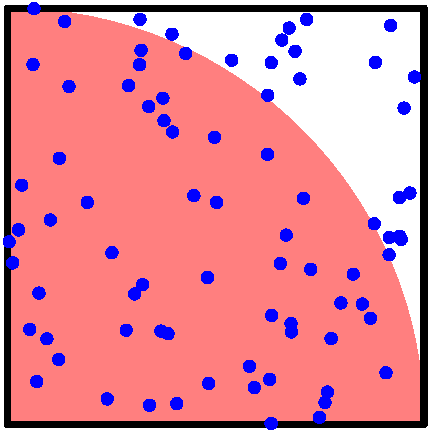
\includegraphics[width=0.9\linewidth]{metapost_pi/pi}
\end{minipage}
\begin{minipage}{0.6\linewidth}
    \[
    P(x,y) = \begin{cases}1 & 0\!<\!x\!<\!1 ~\mbox{ and }~ 0\!<\!y\!<\!1\\
        0 & \mbox{otherwise}
    \end{cases}
    \]

\bigskip

    \[
    %\pi = 4 \int_0^1 \mathrm{d}x \int_0^1 \mathrm{d}y\;\; {\mathbb I}\left((x^2+y^2)<1\right)
    \pi = 4 \iint \Red{{\mathbb I}\left((x^2+y^2)<1\right)} \Blue{P(x,y)} \;\mathrm{d}x\;\mathrm{d}y
    \]
\end{minipage}

\vfill

\begin{verbatim}
octave:1> S=12; a=rand(S,2); 4*mean(sum(a.*a,2)<1)
ans = 3.3333
octave:2> S=1e7; a=rand(S,2); 4*mean(sum(a.*a,2)<1)
ans = 3.1418
\end{verbatim}

%%%%%%%%%%%%%%%%%%%%%%%%%%%%%%%%%%%%%%%%%%%%%%%%%%%%%%%%%%%%%%%%%%%%%%
\myfoilhead{Aside: don't always sample!}

\vfill

%Alan Sokal began a 1996 lecture course on Monte Carlo with:
\begin{quote}
\textsl{``Monte Carlo is an extremely bad method; it should be used only when all
alternative methods are worse.''}
\end{quote}
\vspace*{-0.2in}
\begin{flushright}
    --- Alan Sokal, 1996
\end{flushright}

\vfill

\Green{\bf Example: numerical solutions to (nice) 1D integrals are fast}

% gn = add_call_counter(@(x) sqrt(1-x.^2));
% x = 4*quadl(gn, 0, 1, 0); gn(), fprintf('%10.10g\n', x, pi), (x-pi)
% x = 4*quadl(gn, 0, 1, 1e-6); gn(), fprintf('%10.10g\n', x, pi), (x-pi)
% NO! Because quadl is vectorized need to count function calls more
% carefully.  See ./quadl, for how to do it.

\bigskip

\begin{verbatim}
octave:1> 4 * quadl(@(x) sqrt(1-x.^2), 0, 1, tolerance)
\end{verbatim}

\bigskip

Gives $\pi$ to 6 dp's in 108 evaluations, machine precision in 2598.\\
\Gray{\small (NB Matlab's \texttt{quadl} fails at zero tolerance)}

\vfill

Other lecturers are covering alternatives for higher dimensions.\\
{\small No approx.\ integration method always works. Sometimes Monte Carlo is the best.}

%%%%%%%%%%%%%%%%%%%%%%%%%%%%%%%%%%%%%%%%%%%%%%%%%%%%%%%%%%%%%%%%%%%%%%
\myfoilhead{Eye-balling samples}

\begin{minipage}{0.34\linewidth}
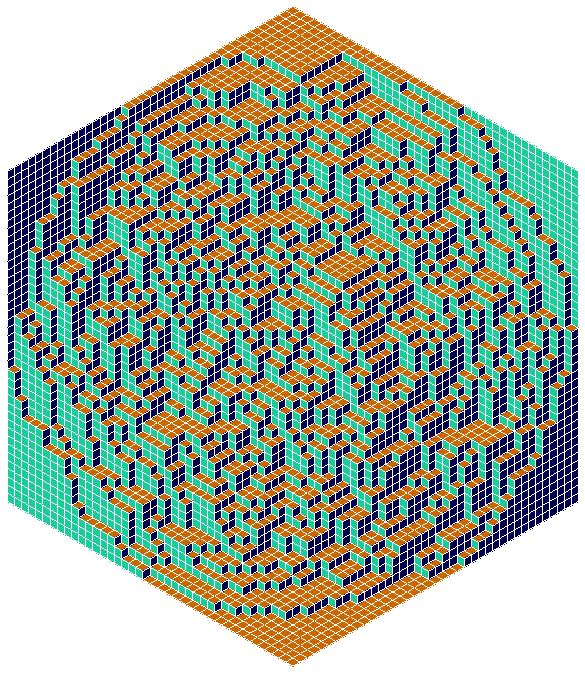
\includegraphics[width=\linewidth]{hexagonbig.pdf}
\end{minipage}~~~
\begin{minipage}{0.7\linewidth}
Sometimes samples are pleasing to look at:\\
{\small (if you're into geometrical combinatorics)}

\vspace*{2cm}
\Gray{\small Figure by Propp and Wilson. Source: MacKay textbook.}
\end{minipage}

\vfill

Sanity check probabilistic modelling assumptions:

\begin{center}\scalebox{0.8}{
\begin{minipage}{\linewidth}
\hspace*{\fill}
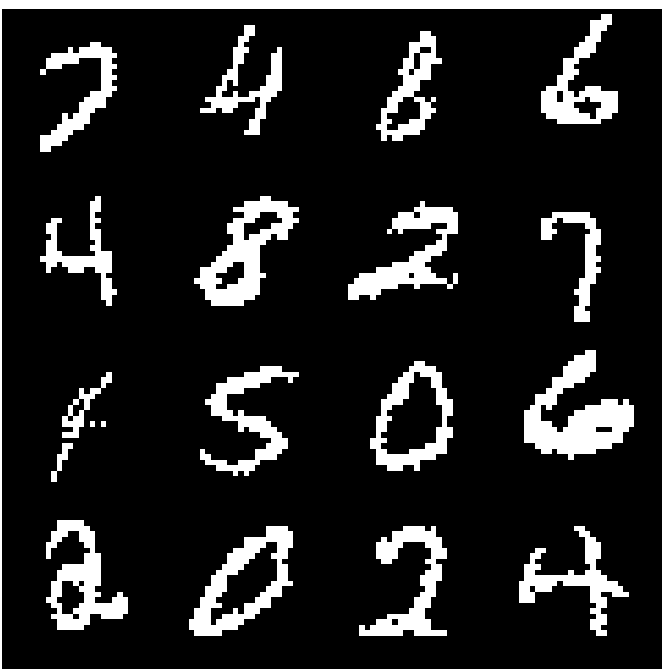
\includegraphics[scale=0.65]{icml_figs/train_samples}
\hspace*{\fill}
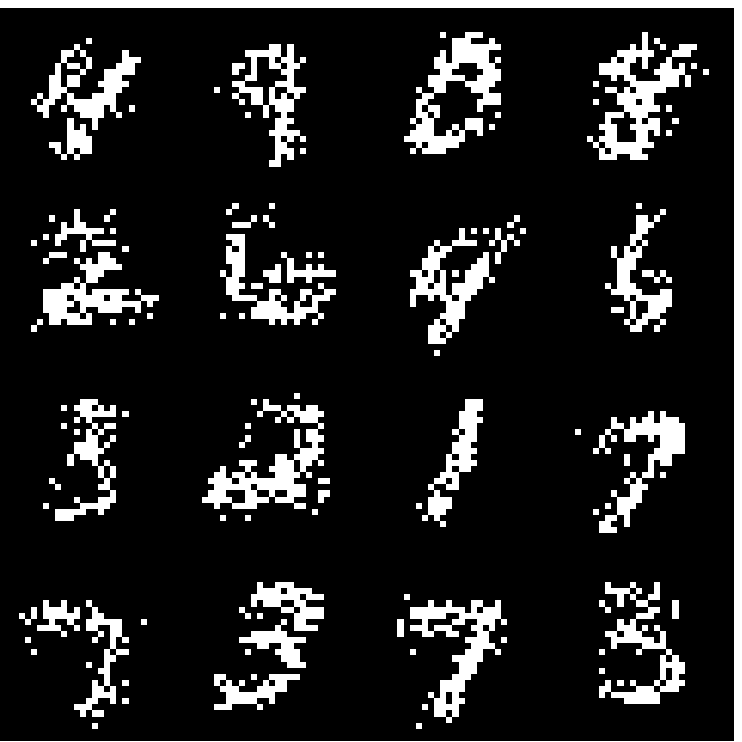
\includegraphics[scale=0.58]{icml_figs/MoB100}
\hspace*{\fill}
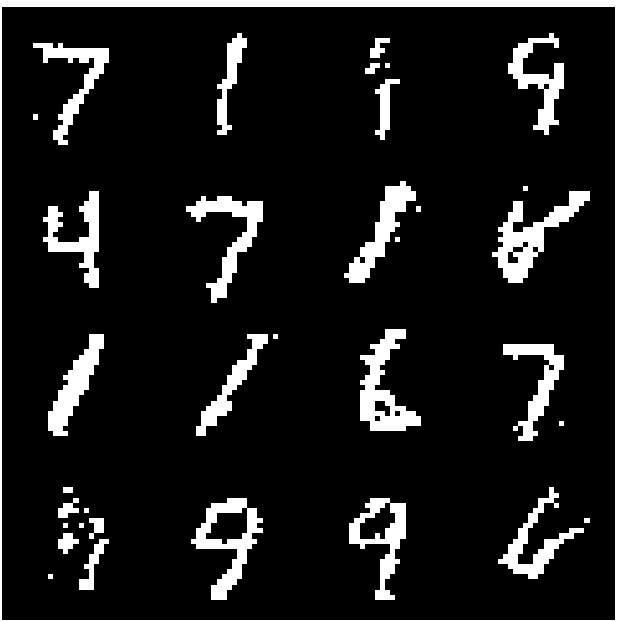
\includegraphics[scale=0.7]{icml_figs/CD25_500_samples}
\hspace*{\fill}
\medskip

\hspace*{2.0cm}\hbox{Data samples}
\hspace*{3.0cm}\hbox{MoB samples}
\hspace*{3.0cm}\hbox{RBM samples}
\end{minipage}}
\end{center}

\vspace*{-0.7cm}

%%%%%%%%%%%%%%%%%%%%%%%%%%%%%%%%%%%%%%%%%%%%%%%%%%%%%%%%%%%%%%%%%%%%%%
\myfoilhead{Monte Carlo and Insomnia}

\vfill

\begin{minipage}{0.43\linewidth}
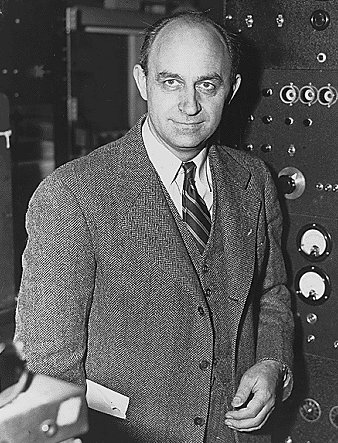
\includegraphics[width=0.9\linewidth]{enrico-fermi}
\end{minipage}
\begin{minipage}{0.56\linewidth}
    \vfill
    {\bf Enrico Fermi} (1901--1954) took great delight in astonishing his
    colleagues with his remakably accurate predictions of experimental
    results\ldots he revealed that his ``guesses'' were really derived from the
    statistical sampling techniques that he used to calculate with whenever
    insomnia struck in the wee morning hours!

    \bigskip

    \begin{flushright}
        {\small ---{\em The beginning of the Monte Carlo method}, N. Metropolis}
    \end{flushright}

    \vfill
\end{minipage}

\vfill

%%%%%%%%%%%%%%%%%%%%%%%%%%%%%%%%%%%%%%%%%%%%%%%%%%%%%%%%%%%%%%%%%%%%%%
\myfoilhead{Sampling from a Bayes net}

\vfill
\Green{\bf Ancestral pass} for directed graphical models:\\[0.1in]
\hspace*{3cm} --- sample each top level variable from its marginal\\[0.1in]
\hspace*{3cm} --- sample each other node from its conditional\\
\hspace*{3cm} \hphantom{---} once its parents have been sampled

\vfill

\begin{minipage}{0.35\linewidth}
    \vspace*{0.5cm}
    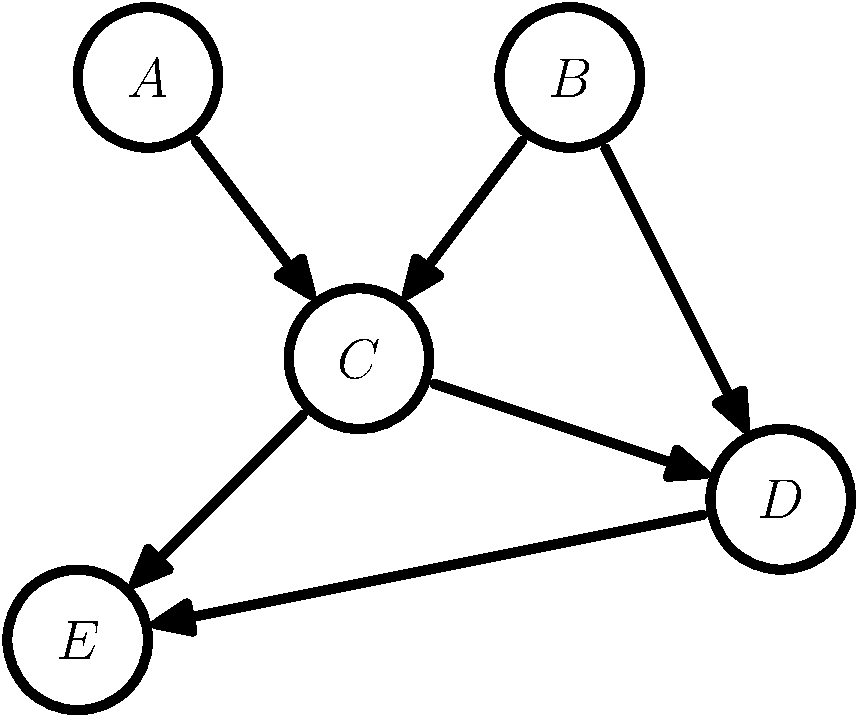
\includegraphics[width=\linewidth]{graphs/graphs0}
\end{minipage}~~~~~~~
\begin{minipage}{0.6\linewidth}
    \Green{\bf Sample:}\\[0.1in]
    $A\sim P(A)$\\
    $B\sim P(B)$\\
    $C\sim P(C\g A,B)$\\
    $D\sim P(D\g B, C)$\\
    $E\sim P(D\g C, D)$
\end{minipage}

\vfill

$P(A,B,C,D,E) = P(A)\,P(B)\,P(C\g A,B)\,P(D\g B,C)\,P(E\g C,D)$

%%%%%%%%%%%%%%%%%%%%%%%%%%%%%%%%%%%%%%%%%%%%%%%%%%%%%%%%%%%%%%%%%%%%%%
\myfoilhead{Sampling the conditionals}

\vspace*{1cm}

\begin{minipage}{0.45\linewidth}
    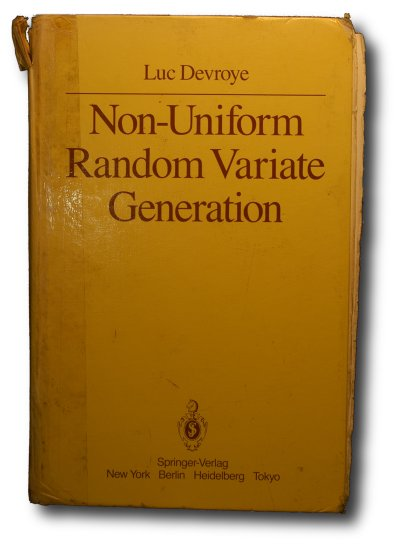
\includegraphics[width=0.95\linewidth]{RNBOOK3}
\end{minipage}
\begin{minipage}{0.54\linewidth}
    \Green{\bf\large Use library routines for\\ univariate distributions}\\
    (and some other special cases)\\[0.6in]

    This book (free online) explains how some of them work\\[0.4in]
    %Second edition ``in the works''
\end{minipage}

\vfill

{\tt http://cg.scs.carleton.ca/\~{}luc/rnbookindex.html}


%%%%%%%%%%%%%%%%%%%%%%%%%%%%%%%%%%%%%%%%%%%%%%%%%%%%%%%%%%%%%%%%%%%%%%
\myfoilhead{Sampling from distributions}

\vspace*{3cm}

%\textbf{Alternative view}:
\Green{\large\bf Draw points uniformly under the curve:}

\bigskip
\bigskip
\bigskip

\centerline{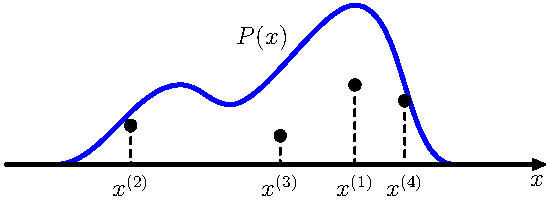
\includegraphics[scale=2.2]{rejection/rejection1}}

\vfill

Probability mass to left of point $\sim\mbox{Uniform[0,1]}$\\[-0.3in]
%Probability mass to left of point still $\sim\mbox{Uniform[0,1]}$\\[-0.3in]
\vfill

%%%%%%%%%%%%%%%%%%%%%%%%%%%%%%%%%%%%%%%%%%%%%%%%%%%%%%%%%%%%%%%%%%%%%%
\myfoilhead{Sampling from distributions}

\vfill

How to convert samples from a Uniform[0,1] generator:

\vfill

\begin{minipage}{0.6\linewidth}
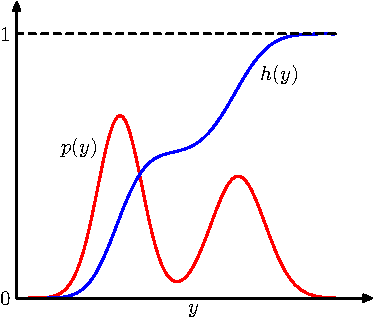
\includegraphics[scale=2.2]{prmlfigs-pdf/Figure11_2}\\[-1cm]
\Gray{\tiny Figure from PRML, Bishop (2006)}
\end{minipage}
\begin{minipage}{0.4\linewidth}

$h(y)=\int_{-\infty}^y p(y') \;\mathrm{d}y'$\\

\bigskip
\bigskip

Draw mass to left of point:\\
\hspace*{1cm}$u\sim\mbox{Uniform[0,1]}$\\

\bigskip

Sample, $y(u) = h^{-1}(u)$
\end{minipage}

\vfill
\vfill

\Red{Although we can't always compute and invert $h(y)$}

\vspace*{-0.5cm}


%%%%%%%%%%%%%%%%%%%%%%%%%%%%%%%%%%%%%%%%%%%%%%%%%%%%%%%%%%%%%%%%%%%%%%%
%\myfoilhead{Sampling from distributions}
%
%\vfill
%
%\textbf{Problem:} cumulative $h(x)$ can be hard to compute and invert\\[0.3cm]
%\hspace*{3cm}$h(x)=\int_{-\infty}^x p(x') \;\mathrm{d}x'$\\[0.3cm]
%%is an integral like the ones we are trying to solve!
%
%\vfill
%
%\textbf{Common situation:}~~~ $\displaystyle p(x) = \frac{\tilde{p}(x)}{\Z}$\\[0.5cm]
%Can evaluate $\tilde{p}(x)$ at any point, but $\Z$ is unknown:\\[0.5cm]
%\hspace*{3cm}--- undirected graphical models: $p(x) = \frac{1}{\Z} \prod_i f_i(x)$\\[0.5cm]
%\hspace*{3cm}--- posterior distributions $p(\theta|\D) = \frac{1}{p(\D)} p(\D|\theta)p(\theta)$
%
%\vfill
%%%%%%%%%%%%%%%%%%%%%%%%%%%%%%%%%%%%%%%%%%%%%%%%%%%%%%%%%%%%%%%%%%%%%%
\myfoilhead{Rejection sampling}

\vspace*{1cm}

% Probably better just saying this:
% {\em To draw a random person in Cambridge, one could select people at random from
% the entire UK and reject anyone not in Cambridge}

Sampling underneath a $\tilde{P}(x)\!\propto\! P(x)$ curve is also valid

\vspace*{2cm}

\hspace*{-1cm}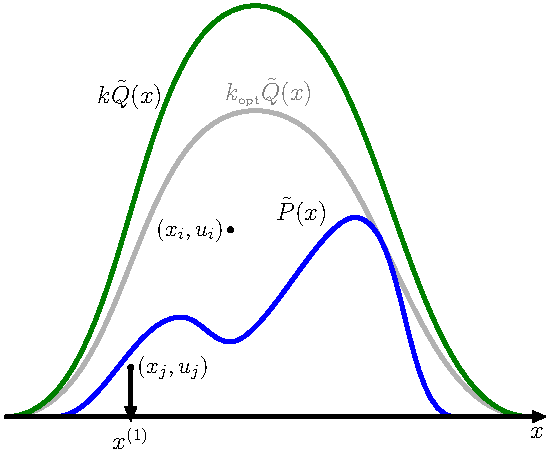
\includegraphics[width=0.65\linewidth]{rejection/rejection0}

\vspace*{-13cm}

\hspace*{0.5\linewidth}\begin{minipage}{0.55\linewidth}
    Draw underneath a simple\\curve $k \tilde{Q}(x)\ge \tilde{P}(x)$:\\[0.1in]
\hspace*{2cm} -- Draw $x\sim Q(x)$\\
\hspace*{2cm} -- height $u\sim\mbox{Uniform}[0,k\tilde{Q}(x)]$\\

Discard the point if above $\tilde{P}$,\\i.e.\ if $u>\tilde{P}(x)$

\vfill
\end{minipage}

%%%%%%%%%%%%%%%%%%%%%%%%%%%%%%%%%%%%%%%%%%%%%%%%%%%%%%%%%%%%%%%%%%%%%%
\myfoilhead{Importance sampling}

\vfill

Computing $\tilde{P}(x)$ and $\tilde{Q}(x)$, then \emph{throwing $x$ away} seems wasteful\\
Instead rewrite the integral as an \Blue{expectation under $Q$}:
\[
\begin{split}
    \int f(x)P(x) \;\mathrm{d}x &\;=\; \Blue{\int} f(x)\frac{P(x)}{Q(x)} \Blue{Q(x) \;\mathrm{d}x}, \qquad \mbox{\small $(Q(x)>0\mbox{ if }P(x)>0)$}\\
    &\;\approx\; \Blue{\frac{1}{S} \sum_{s=1}^S} f(x^{\Blue{(s)}})\frac{P(x^{\Blue{(s)}})}{Q(x^{\Blue{(s)}})}\Blue{, \quad x^{(s)}\sim Q(x)}
\end{split}
\]
%Unbiased, but $Q(x)$ must not be zero (or very small) when $P(x)>0$\\

\vfill

This is just simple Monte Carlo again, so it is unbiased.

%Unbiased; but light-tailed $Q(x)$ can give the estimator infinite variance\\
%\hspace*{2cm} \dots and you might not notice.

\vfill

Importance sampling applies when the integral is not an expectation.\\
Divide and multiply any integrand by a convenient distribution.

%%%%%%%%%%%%%%%%%%%%%%%%%%%%%%%%%%%%%%%%%%%%%%%%%%%%%%%%%%%%%%%%%%%%%%
\myfoilhead{Importance sampling (2)}

%\vspace*{1cm}

\vfill

Previous slide assumed we could evaluate $P(x)=\tilde{P}(x)/\Z_P$
\[
\begin{split}
    \int f(x)P(x) \;\mathrm{d}x &\;\approx\; \Red{\frac{\Z_Q}{\Z_P}}~\frac{1}{S} \sum_{s=1}^S f(x^{(s)})%
    \underset{\mathclap{\mbox{\large $\tilde{r}^{(s)}$}}}{\underbrace{\frac{\tilde{P}(x^{(s)})}{\tilde{Q}(x^{(s)})}}}, ~~x^{(s)}\sim Q(x)\\
    & \;\approx\; \LightGray{\cancel{\frac{1}{S}}}\sum_{s=1}^S f(x^{(s)}) \frac{\tilde{r}^{(s)}}{\LightGray{\cancel{\frac{1}{S}}}\Red{\sum_{s'} \tilde{r}^{(s')}}}
    \;\equiv\;\sum_{s=1}^S f(x^{(s)}) w^{(s)}
\end{split}
\]

This estimator is \Green{\bf consistent} but \Green{\bf biased}

\vfill
\Green{\bf Exercise:} Prove that ${\Z_P}/{\Z_Q}\approx \frac{1}{S}\sum_s \tilde{r}^{(s)}$
% \[
% \frac{\Z_P}{\Z_Q}
% = \int \frac{\Z_P}{\Z_Q} P(x) \;\mathrm{d}x
% = \int \frac{\tilde{P}(x)}{\Z_Q} \;\mathrm{d}x
% = \int \frac{\tilde{P}(x)}{\tilde{Q}(x)} Q(x) \;\mathrm{d}x
% \approx \frac{1}{S} \sum_{s=1}^S \frac{\tilde{P}(x^{(s)})}{\tilde{Q}(x^{(s)})}, ~x^{(s)}\sim Q(x)
% \]

% %%%%%%%%%%%%%%%%%%%%%%%%%%%%%%%%%%%%%%%%%%%%%%%%%%%%%%%%%%%%%%%%%%%%%%
% \myfoilhead{Simple Monte Carlo's problem}
% 
% \vspace*{1cm}
% 
% We only know how to sample from simple distributions\\
% Yet probability mass must lie at all large parts of the integrand
% 
% \vfill
% 
% [Life in high dimensions]
% 
% \vfill

%%%%%%%%%%%%%%%%%%%%%%%%%%%%%%%%%%%%%%%%%%%%%%%%%%%%%%%%%%%%%%%%%%%%%%
\myfoilhead{Summary so far}

\vfill

\begin{itemize}
    \setlength{\itemsep}{10pt}
    \setlength{\parskip}{10pt}
    \setlength{\parsep}{0cm}

\item Sums and integrals, often expectations, occur frequently in statistics

\item \Green{\bf Monte Carlo} approximates expectations with a sample average

\item \Green{\bf Rejection sampling} draws samples from complex distributions

\item \Green{\bf Importance sampling} applies Monte Carlo to `any' sum/integral

\end{itemize}

\vfill
\vfill

% If our $Q(x)$ distribution is a poor fit to $P(x)$:\\[0.3cm]
% \hspace*{2cm}--- rejection samplers almost always reject\\[0.3cm]
% % (large $k$ needed)\\[0.3cm]
% \hspace*{2cm}--- importance sampling has large or infinite variance\\[0.3cm]
% In high dimensions finding a good $Q(x)$ is hard. What then?

%%%%%%%%%%%%%%%%%%%%%%%%%%%%%%%%%%%%%%%%%%%%%%%%%%%%%%%%%%%%%%%%%%%%%%
\myfoilhead{Application to large problems}

\vfill

We often can't decompose $P(X)$ into low-dimensional conditionals
% like a prior directed graphical model

\vfill

\begin{minipage}{0.75\linewidth}
\Green{\bf Undirected graphical models:} $P(x) = \frac{1}{\Z} \prod_i f_i(x)$
\end{minipage}
\begin{minipage}{0.3\linewidth}
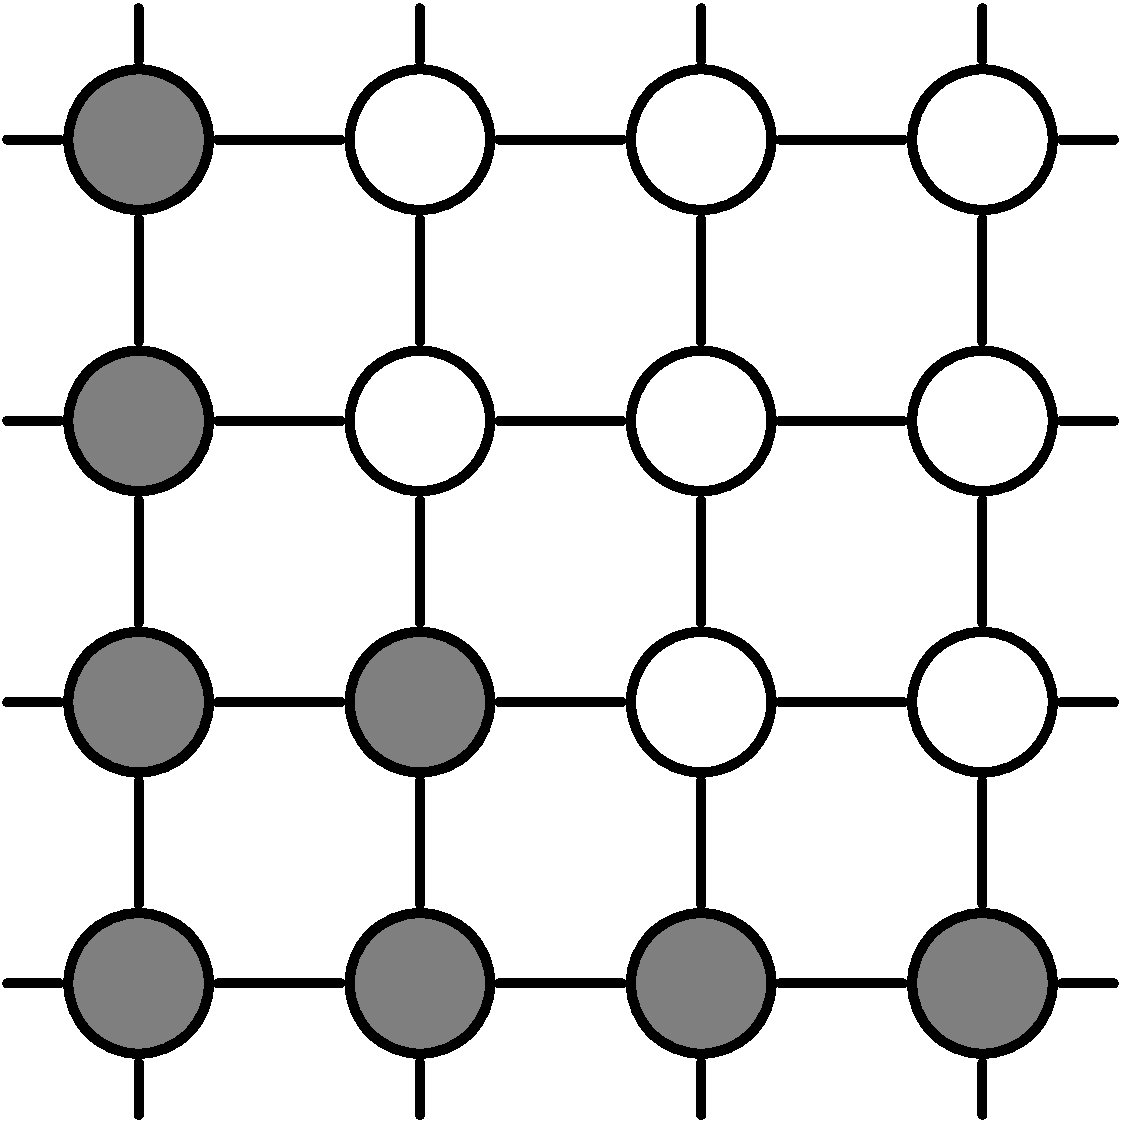
\includegraphics[scale=0.3]{figures/figure5}
\end{minipage}

\vfill

\begin{minipage}{0.35\linewidth}
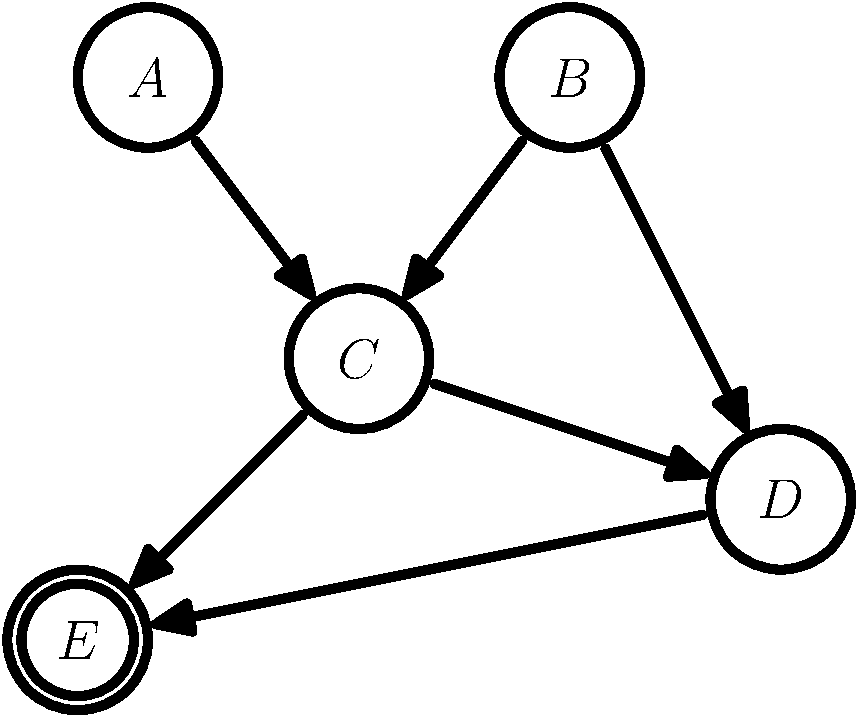
\includegraphics[width=\linewidth]{graphs/graphs1}
\end{minipage}~~~
\begin{minipage}{0.65\linewidth}
\Green{\bf Posterior} of a directed graphical model\\

$\displaystyle P(A,B,C,D\g E) = \frac{P(A,B,C,D,E)}{P(E)}$
\end{minipage}

\begin{flushright}
\Red{We often don't know $\Z$ or $P(E)$}
\end{flushright}

\vspace*{-0.5cm}

%%%%%%%%%%%%%%%%%%%%%%%%%%%%%%%%%%%%%%%%%%%%%%%%%%%%%%%%%%%%%%%%%%%%%%
\myfoilhead{Application to large problems}

\vfill

\Green{\bf Rejection \& importance sampling scale badly with dimensionality}\\

Example:
\[
P(x) = \N(0,\,\I),~~~Q(x) = \N(0,\,\sigma^2\I)
\]
\vfill

% P = (2pi)^(-D/2) exp(-0.5*x^2)
% Q = (2pi sigma^2)^(-D/2) exp(-0.5*x^2 / sigma^2)
%
% P/Q = sigma^D exp(-0.5*x^2*(1 - 1/sigma^2))
% c = max_x P/Q = sigma^D if sigma^2 >= 1
%                 inf if sigma^2<1
%
% Fraction of proposals rejected = (c-1)/c = 1 - 1/c
% Fraction of proposals accepted = 1/c

\Green{\bf Rejection sampling:}\\[0.1in]
Requires $\sigma\geq 1$. Fraction of proposals accepted $= \sigma^{-D}$\\

\vfill

% var(P/Q) = \int (P/Q)^2 Q - \int (P/Q) Q
%          = \int P^2/Q - 1
%          = (2pi)^(-D/2) sigma^D \prod_d \int exp(-x^2*(1 - 1/(2*sigma^2))) - 1
%
% now int exp(-0.5 * z^2 / sigma^2) = sqrt(2*pi*sigma^2)
%     int exp(-a * z^2) = sqrt(pi/a),            a = 0.5/sigma^2; sigma^2 = 0.5/a
%
%          = (2pi)^(-D/2) sigma^D pi^(D/2) (1-1/(2*sigma^2))^(-D/2)
%          = (2)^(-D/2) sigma^D (1-1/(2*sigma^2))^(-D/2)

\Green{\bf Importance sampling:}\\[0.1in]
Variance of importance weights $ = \left(\frac{\sigma^2}{2-1/\sigma^2}\right)^{D/2} - 1$\\[0.2in]
Infinite / undefined variance if $\sigma \leq 1/\sqrt{2}$

%%%%%%%%%%%%%%%%%%%%%%%%%%%%%%%%%%%%%%%%%%%%%%%%%%%%%%%%%%%%%%%%%%%%%%
\myfoilhead{Importance sampling weights}

\vfill

\begin{minipage}{0.19\linewidth}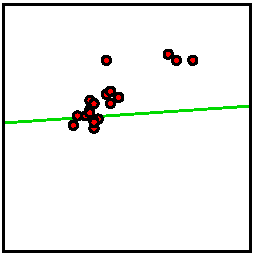
\includegraphics[width=\linewidth]{is_demo/figures/is_demo01}
\small \centerline{$w=$\texttt{0.00548}}\\
\end{minipage}
\begin{minipage}{0.19\linewidth}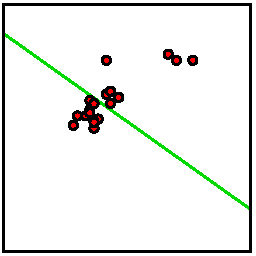
\includegraphics[width=\linewidth]{is_demo/figures/is_demo02}
\small \centerline{$w=$\texttt{1.59e-08}}\\
\end{minipage}
\begin{minipage}{0.19\linewidth}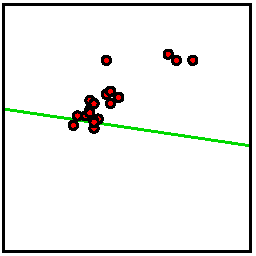
\includegraphics[width=\linewidth]{is_demo/figures/is_demo03}
\small \centerline{$w=$\texttt{9.65e-06}}\\
\end{minipage}
\begin{minipage}{0.19\linewidth}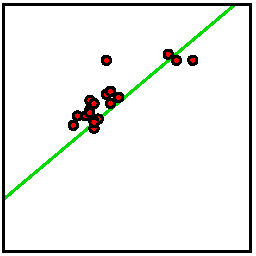
\includegraphics[width=\linewidth]{is_demo/figures/is_demo04}
\small \centerline{$w=$\texttt{0.371}}\\
\end{minipage}
\begin{minipage}{0.19\linewidth}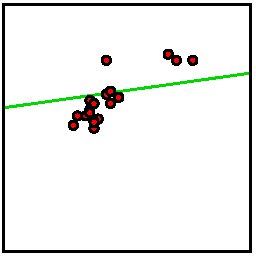
\includegraphics[width=\linewidth]{is_demo/figures/is_demo05}
\small \centerline{$w=$\texttt{0.103}}\\
\end{minipage}

\vfill

\begin{minipage}{0.19\linewidth}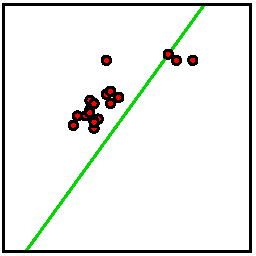
\includegraphics[width=\linewidth]{is_demo/figures/is_demo06}
\small \centerline{$w=$\texttt{1.01e-08}}\\
\end{minipage}
\begin{minipage}{0.19\linewidth}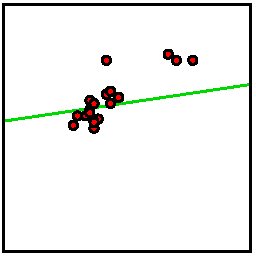
\includegraphics[width=\linewidth]{is_demo/figures/is_demo07}
\small \centerline{$w=$\texttt{0.111}}\\
\end{minipage}
\begin{minipage}{0.19\linewidth}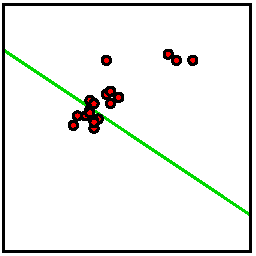
\includegraphics[width=\linewidth]{is_demo/figures/is_demo08}
\small \centerline{$w=$\texttt{1.92e-09}}\\
\end{minipage}
\begin{minipage}{0.19\linewidth}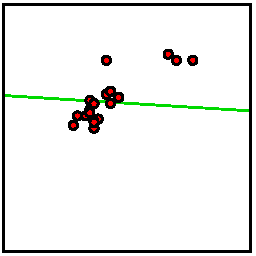
\includegraphics[width=\linewidth]{is_demo/figures/is_demo09}
\small \centerline{$w=$\texttt{0.0126}}\\
\end{minipage}
\begin{minipage}{0.19\linewidth}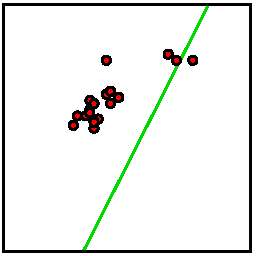
\includegraphics[width=\linewidth]{is_demo/figures/is_demo10}
\small \centerline{$w=$\texttt{1.1e-51}}\\
\end{minipage}

\vfill

%%%%%%%%%%%%%%%%%%%%%%%%%%%%%%%%%%%%%%%%%%%%%%%%%%%%%%%%%%%%%%%%%%%%%%
\myfoilhead{Metropolis algorithm}

\vfill

\begin{minipage}{0.19\linewidth}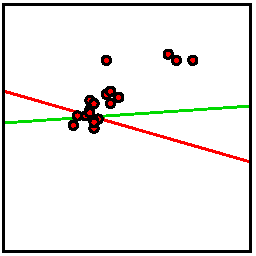
\includegraphics[width=\linewidth]{is_demo/figures/is_demo12}
\end{minipage}
\begin{minipage}{0.19\linewidth}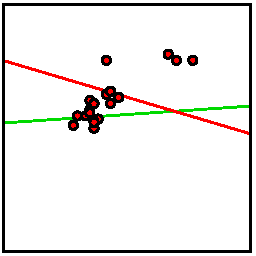
\includegraphics[width=\linewidth]{is_demo/figures/is_demo13}
\end{minipage}
\begin{minipage}{0.19\linewidth}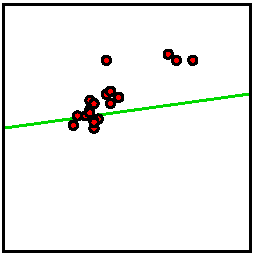
\includegraphics[width=\linewidth]{is_demo/figures/is_demo14}
\end{minipage}
\begin{minipage}{0.19\linewidth}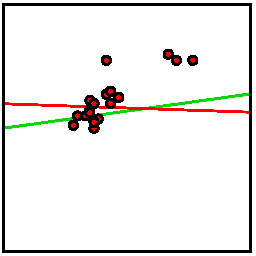
\includegraphics[width=\linewidth]{is_demo/figures/is_demo15}
\end{minipage}
\begin{minipage}{0.19\linewidth}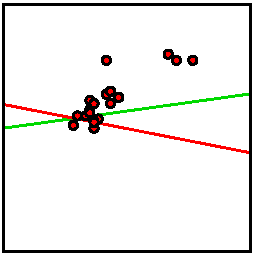
\includegraphics[width=\linewidth]{is_demo/figures/is_demo16}
\end{minipage}
\begin{minipage}{0.19\linewidth}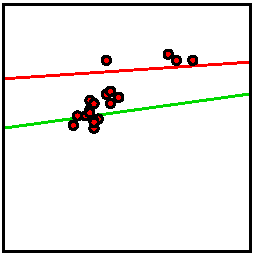
\includegraphics[width=\linewidth]{is_demo/figures/is_demo17}
\end{minipage}
\begin{minipage}{0.19\linewidth}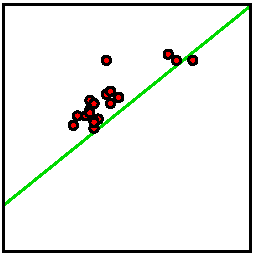
\includegraphics[width=\linewidth]{is_demo/figures/is_demo18}
\end{minipage}
\begin{minipage}{0.19\linewidth}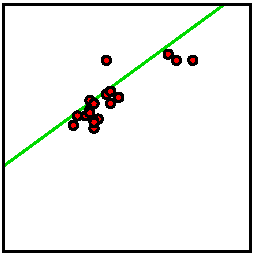
\includegraphics[width=\linewidth]{is_demo/figures/is_demo19}
\end{minipage}
\begin{minipage}{0.19\linewidth}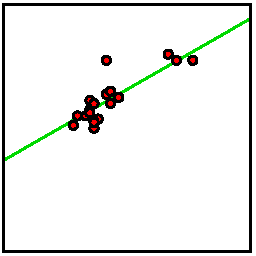
\includegraphics[width=\linewidth]{is_demo/figures/is_demo20}
\end{minipage}
\begin{minipage}{0.19\linewidth}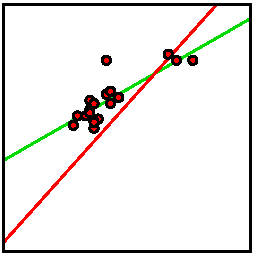
\includegraphics[width=\linewidth]{is_demo/figures/is_demo21}
\end{minipage}

\vfill

\begin{minipage}{0.7\linewidth}
\begin{itemize}
    \setlength{\itemsep}{5pt}
    \setlength{\parskip}{5pt}
    \setlength{\parsep}{0cm}
\item Perturb parameters: $Q(\theta';\theta)$, e.g.\ $\N(\theta,\sigma^2)$
\item Accept with probability $\displaystyle\kern6pt\min\kern-6pt\left(1,\; \frac{\tilde{P}(\theta'|\D)}{\tilde{P}(\theta|\D)}\right)$
\item Otherwise \textbf{keep old parameters}
\end{itemize}
\end{minipage}
\begin{minipage}{0.3\linewidth}
    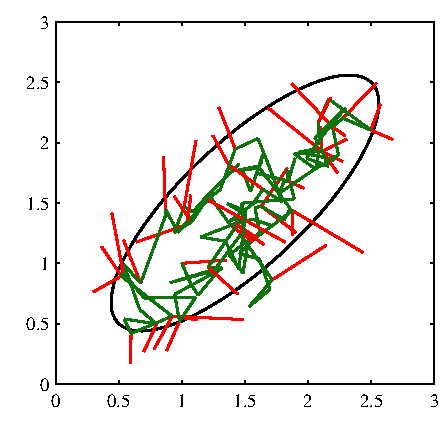
\includegraphics[width=\linewidth]{prmlfigs-pdf/Figure11_9}\\[-1cm]
    \Gray{\tiny This subfigure from PRML, Bishop (2006)}
\end{minipage}

\vspace*{-0.5cm}
\Gray{\tiny Detail: Metropolis, as stated, requires $Q(\theta';\theta) = Q(\theta;\theta')$}

%%%%%%%%%%%%%%%%%%%%%%%%%%%%%%%%%%%%%%%%%%%%%%%%%%%%%%%%%%%%%%%%%%%%%%
\myfoilhead{Markov chain Monte Carlo}

\vspace*{1.3cm}

\Green{\bf Construct a biased random walk that explores target dist $P^\star(x)$}\\

Markov steps, $x_t\sim T(x_t\la x_{t-1})$

\vfill

\centerline{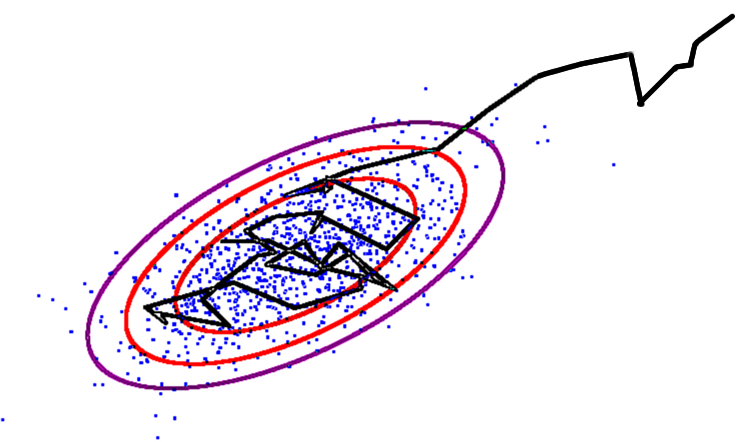
\includegraphics[scale=2]{mcmc2}}

\vfill
\Red{MCMC gives approximate, correlated samples from $P^\star(x)$}

%%%%%%%%%%%%%%%%%%%%%%%%%%%%%%%%%%%%%%%%%%%%%%%%%%%%%%%%%%%%%%%%%%%%%%
\myfoilhead{Transition operators}

\vspace*{1cm}

%\Green{\bf $T(x'\la x)=$ probability of moving from current state $x$ to state $x'$}\\[0.2in]

\Green{\bf Discrete example}\\[-0.1in]
{\small \[
P^\star=\left(\begin{matrix}
    3/5 \\
    1/5 \\
    1/5
\end{matrix}\right) 
\qquad
T = \left(\begin{matrix}
    2/3 & 1/2 & 1/2 \\
    1/6 &  0  & 1/2 \\
    1/6 & 1/2 &  0
\end{matrix}\right) \qquad T_{ij} = T(x_i\la x_j)
\]}

\vfill
\vspace*{0.3cm}

$P^\star$ is an \Green{\bf invariant distribution} of $T$ because $TP^\star\te P^\star$, i.e.
\[
\sum_x T(x'\la x) P^\star(x) = P^\star(x')
\]

\vspace*{-0.5cm}
%\Green{\bf Transition operators are easily combined}:\\
%if $RP=P$ then $(RT)P=R(TP)=RP=P$

\vfill

Also $P^\star$ is \emph{the} \Green{\bf equilibrium distribution} of $T$:\\[0.3cm]
\hspace*{4cm}$ \mbox{To machine precision: } T^{100} \mbox{\tiny $\left(\begin{matrix}1\\0\\0\end{matrix}\right)$}=
\mbox{\tiny $\left(\begin{matrix}3/5\\1/5\\1/5\end{matrix}\right)$} = P^\star$\\[0.3cm]

\vfill

\emph{Ergodicity} requires: $T^K(x'\la x)\!>\!0$ for all $x':P^\star(x')>0$, for some \rlap{$K$}

%%%%%%%%%%%%%%%%%%%%%%%%%%%%%%%%%%%%%%%%%%%%%%%%%%%%%%%%%%%%%%%%%%%%%%%
%\myfoilhead{Detailed balance}
%
%\vfill
%
%Detailed balance means $~\ra x\ra x'$ and $~\ra x'\ra x$ are equally probable:
%\[
%T(x'\la x) P^\star(x) \;=\; T(x\la x') P^\star(x')
%\]
%%``Like Bayes' rule'', but don't write $T(x'|x)$; use $T(x';x)$ or $T(x'\la x)$\\[0.2in]
%
%Summing both sides over $x$:\\[-0.2in]
%\[
%\sum_x T(x'\la x) P^\star(x) \;=\; P^\star(x') \LightGray{\cancelto{1}{\sum_x T(x\la x')}}
%\]\\[-0.1in]
%\Green{\bf detailed balance implies the invariant condition}
%
%\vfill
%\vfill
%Enforcing detailed balance is easy: it only involves isolated pairs

%%%%%%%%%%%%%%%%%%%%%%%%%%%%%%%%%%%%%%%%%%%%%%%%%%%%%%%%%%%%%%%%%%%%%%
\myfoilhead{Detailed Balance}

\vspace*{1cm}

Detailed balance means $\,\ra x\ra x'\,$ and $\,\ra x'\ra x$ are equally probable:
\begin{center}
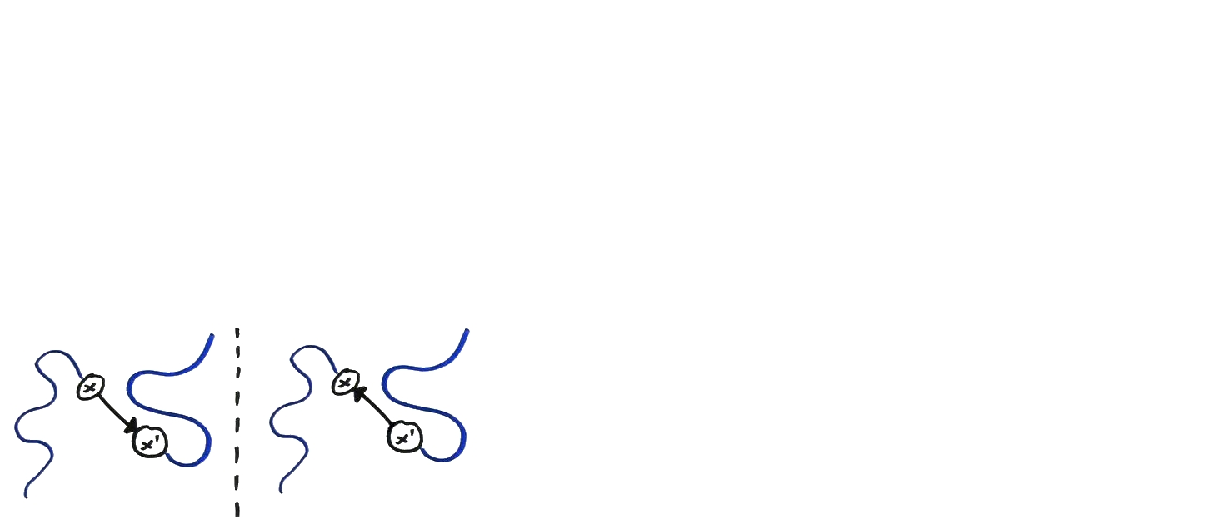
\includegraphics[width=0.7\linewidth]{mcmc_basics/detailedbalance2}

%\vspace*{1cm}
%\Gray{\large $T(y\leftarrow x)P^\star(x) = T(x\leftarrow y)P^\star(y)$}\\
$T(x'\leftarrow x)P^\star(x) = T(x\leftarrow x')P^\star(x')$

%\vspace*{1cm}
%
%\Gray{\large ``Like Bayes rule''}
\end{center}

\vfill

\Green{\bf Detailed balance implies the invariant condition:}\\[-0.2in]
\[
\sum_x T(x'\la x) P^\star(x) \;=\; P^\star(x') \LightGray{\cancelto{1}{\sum_x T(x\la x')}}
\]%\\[-0.1in]

\bigskip
%\vfill
Enforcing detailed balance is easy: it only involves isolated pairs

\vspace*{-0.5cm}

%%%%%%%%%%%%%%%%%%%%%%%%%%%%%%%%%%%%%%%%%%%%%%%%%%%%%%%%%%%%%%%%%%%%%%
\myfoilhead{Reverse operators}

%\vspace*{1cm}
\vfill

\newcommand{\tT}{\widetilde{T}}
\newcommand{\sd}{P^\star}

If $T$ satisfies stationarity, we can define a \emph{reverse operator}
\[
    \tT(x\la x') \propto T(x'\la x)\,\sd(x) =
        \frac{T(x'\la x)\,\sd(x)}{\sum_x T(x'\la x)\,\sd(x)} =
        \frac{T(x'\la x)\,\sd(x)}{\sd(x')} .
\]

\vfill

\Green{\bf Generalized balance condition:}
\[
T(x'\la x) P^\star(x) \;=\; \tT(x\la x') P^\star(x')
\]
also implies the invariant condition \emph{and is necessary}.

\vfill

Operators satisfying detailed balance are their own reverse operator.

%%%%%%%%%%%%%%%%%%%%%%%%%%%%%%%%%%%%%%%%%%%%%%%%%%%%%%%%%%%%%%%%%%%%%%
\myfoilhead{Metropolis--Hastings}

\vfill

\Green{\bf Transition operator}\\[-0.6in]
\begin{itemize}
    \setlength{\itemsep}{5pt}
    \setlength{\parskip}{5pt}
    \setlength{\parsep}{0cm}
\item Propose a move from the current state $Q(x';x)$, e.g.\ $\N(x,\sigma^2)$
\item Accept with probability $\kern3pt\min\kern-6pt\left(1,\; \frac{P(x')Q(x;x')}{P(x)Q(x';x)}\right)$
\item Otherwise next state in chain is a copy of current state
\end{itemize}

\bigskip

\Green{\bf Notes}\\[-0.6in]
\begin{itemize}
    \setlength{\itemsep}{5pt}
    \setlength{\parskip}{5pt}
    \setlength{\parsep}{0cm}
\item Can use $\tilde{P}\propto P(x)$; normalizer cancels in acceptance ratio
\item Satisfies detailed balance {\scriptsize (shown below)}
\item $Q$ must be chosen to fulfill the other technical requirements
\end{itemize}

\vfill

\hrule
\vspace*{0.2in}
{\tiny$\displaystyle%
P(x)\cdot T(x'\la x) = P(x)\cdot Q(x';x)\min\!\left(1,\; \frac{P(x')Q(x;x')}{P(x)Q(x';x)}\right)%
= \min\!\left(P(x)Q(x';x),\;P(x')Q(x;x')\right)$\\
$\displaystyle%
\phantom{P(x)\cdot T(x'\la x) = P(x)\cdot Q(x';x)\min\!\left(1,\; \frac{P(x')Q(x;x')}{P(x)Q(x';x)}\right)}%
= P(x')\cdot Q(x;x')\min\!\left(1,\; \frac{P(x)Q(x';x)}{P(x')Q(x;x')}\right)
= P(x')\cdot T(x\la x')$}

\vspace*{-0.5cm}


%%%%%%%%%%%%%%%%%%%%%%%%%%%%%%%%%%%%%%%%%%%%%%%%%%%%%%%%%%%%%%%%%%%%%%
\myfoilhead{Matlab/Octave code for demo}

\vfill

{\small
\begin{verbatim}
function samples = dumb_metropolis(init, log_ptilde, iters, sigma)

D = numel(init);
samples = zeros(D, iters);

state = init;
Lp_state = log_ptilde(state);
for ss = 1:iters
    % Propose
    prop = state + sigma*randn(size(state));
    Lp_prop = log_ptilde(prop);
    if log(rand) < (Lp_prop - Lp_state)
        % Accept
        state = prop;
        Lp_state = Lp_prop;
    end
    samples(:, ss) = state(:);
end
\end{verbatim}}

\vfill

%%%%%%%%%%%%%%%%%%%%%%%%%%%%%%%%%%%%%%%%%%%%%%%%%%%%%%%%%%%%%%%%%%%%%%
\myfoilhead{Step-size demo}

\vfill

\Green{\bf Explore $\N(0,1)$ with different step sizes $\sigma$}

\bigskip

{\small
% Including this is confusing:
%function samples = dumb_metropolis(init, log_ptilde, iters, sigma)
\begin{verbatim}
sigma = @(s) plot(dumb_metropolis(0, @(x) -0.5*x*x, 1e3, s));
\end{verbatim}}

\vfill \raisebox{2.3cm}{\texttt{sigma(0.1)\phantom{0}}}~~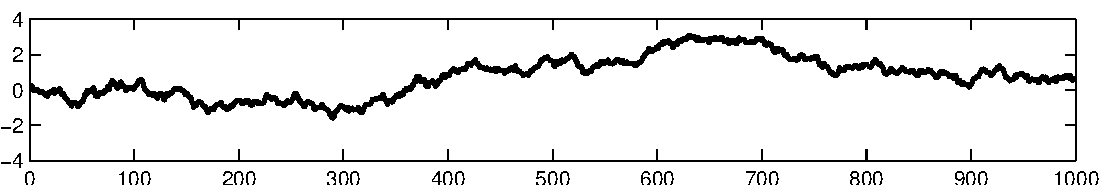
\includegraphics{mh_stepsize_demo/sigma01}

\vspace*{-2cm}
{\small 99.8\% accepts}
\vspace*{1cm}

\vfill \raisebox{2.3cm}{\texttt{sigma(1)\phantom{0.0}}}~~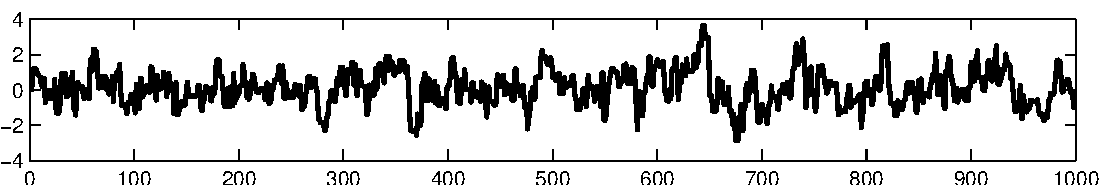
\includegraphics{mh_stepsize_demo/sigma1}

\vspace*{-2cm}
{\small 68.4\% accepts}
\vspace*{1cm}

\vfill \raisebox{2.3cm}{\texttt{sigma(100)\phantom{.}}}~~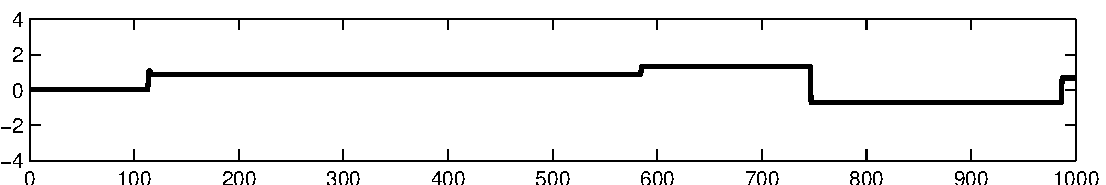
\includegraphics{mh_stepsize_demo/sigma100}

\vspace*{-2cm}
{\small 0.5\% accepts}

% runme2
%ans =
%    0.9980
%ans =
%    0.9489
%ans =
%    0.6837
%ans =
%    0.0050

%%%%%%%%%%%%%%%%%%%%%%%%%%%%%%%%%%%%%%%%%%%%%%%%%%%%%%%%%%%%%%%%%%%%%%
\myfoilhead{Metropolis limitations}

\vfill

\begin{minipage}{0.5\textwidth}
    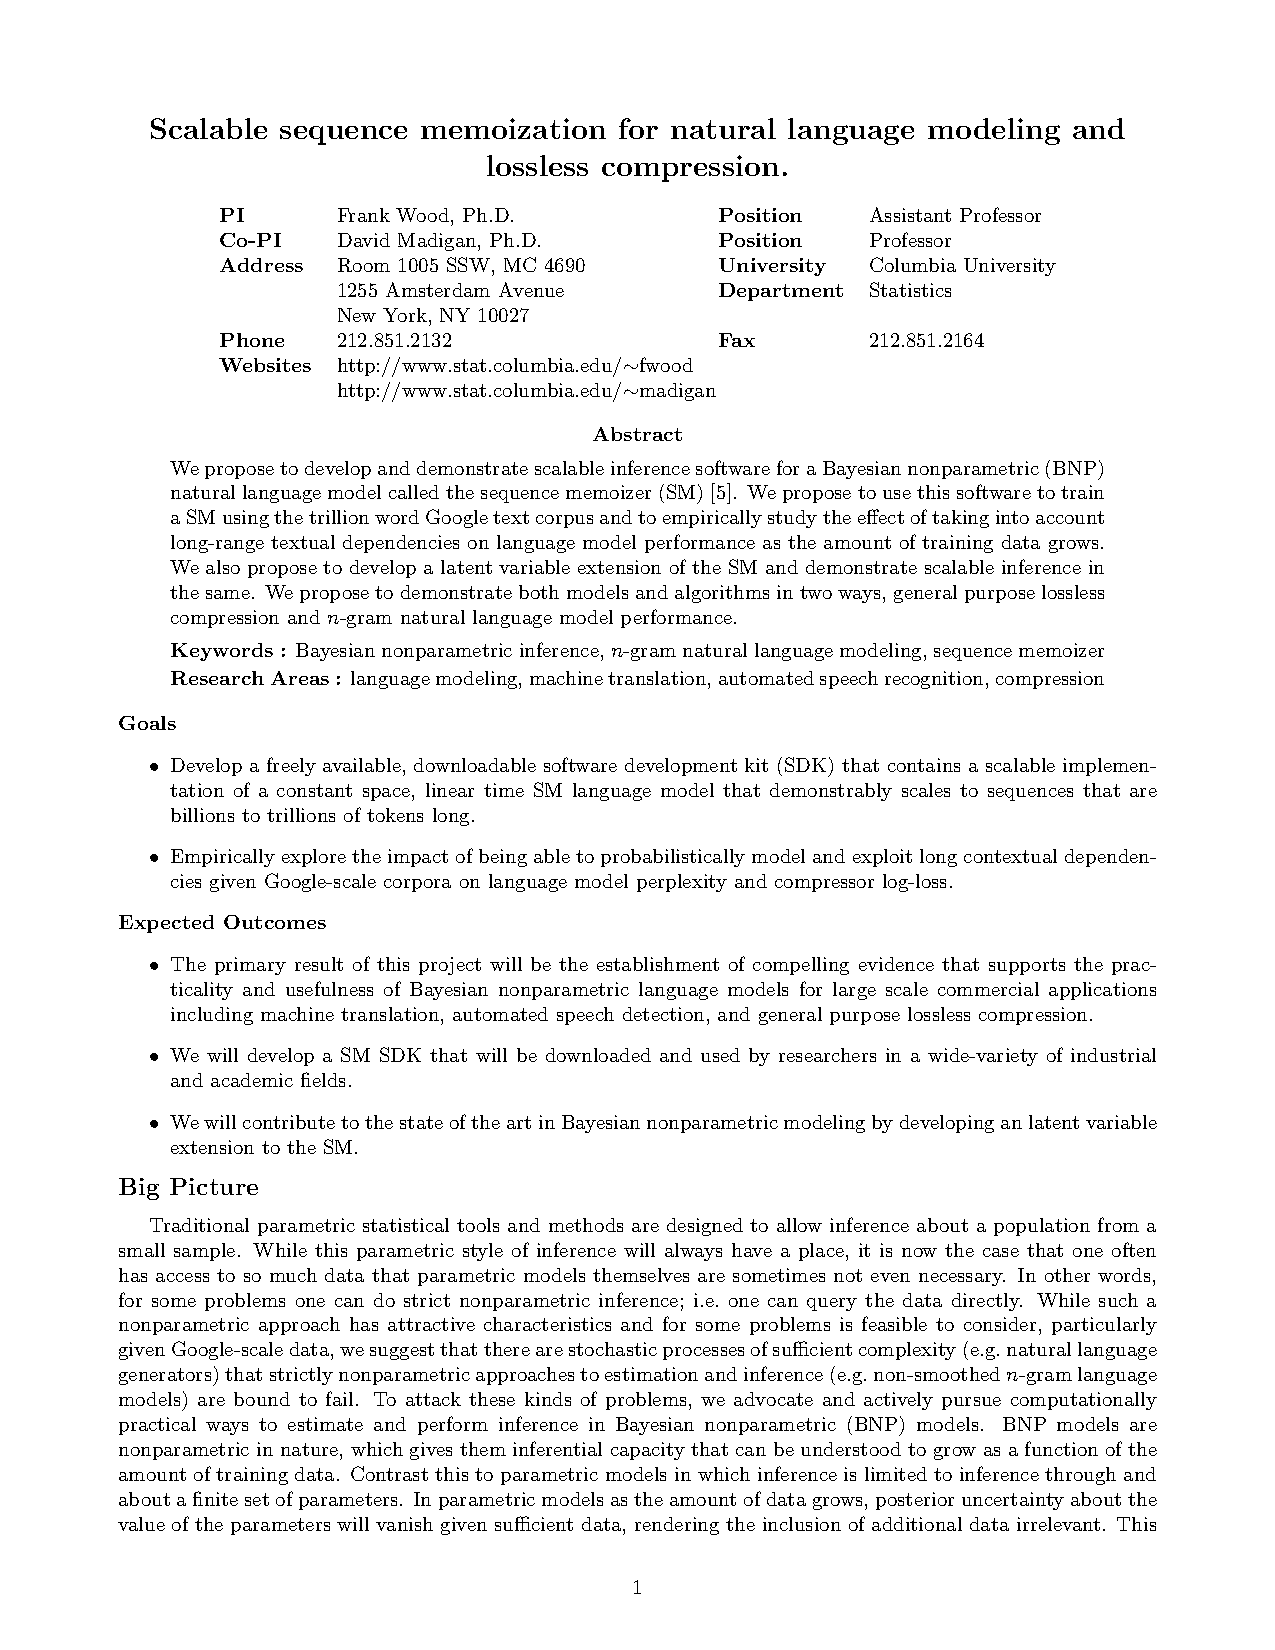
\includegraphics[width=0.95\textwidth]{proposal}
\end{minipage}
\begin{minipage}{0.49\textwidth}
    Generic proposals use\\$Q(x';x)=\N(x,\sigma^2)$\\

    \Green{\bf $\sigma$ large $\rightarrow$ many rejections}\\

    \Green{\bf $\sigma$ small $\rightarrow$ slow diffusion:}\\
    $\sim\!(L/\sigma)^2$ iterations required
\end{minipage}

\vfill

%\Red{\small Adapted from MacKay (2003)}


%%%%%%%%%%%%%%%%%%%%%%%%%%%%%%%%%%%%%%%%%%%%%%%%%%%%%%%%%%%%%%%%%%%%%%
\myfoilhead{Combining operators}

\vfill
A sequence of operators, each with $P^\star$ invariant:\\[-0.2in]

\hspace*{-1cm}\begin{minipage}{0.3\linewidth}
\[
\begin{split}
x_0 &\sim P^\star(x)\\
x_1 &\sim T_a(x_1\la x_0)\\
x_2 &\sim T_b(x_2\la x_1)\\
x_3 &\sim T_c(x_3\la x_2)\\
&\cdots
\end{split}
\]
\end{minipage}
\hspace*{1cm}
\begin{minipage}{0.7\linewidth}
\[
\begin{split}
    \mbox{\phantom{$P^\star(x)$}} &\\
P(x_1) &\;=\; \textstyle \sum_{x_0} T_a(x_1\la x_0) P^\star(x_0) \;=\; P^\star(x_1)\\
P(x_2) &\;=\; \textstyle \sum_{x_1} T_b(x_2\la x_1) P^\star(x_1) \;=\; P^\star(x_2)\\
P(x_3) &\;=\; \textstyle \sum_{x_1} T_c(x_3\la x_2) P^\star(x_2) \;=\; P^\star(x_3)\\
&\cdots
\end{split}
\]
\end{minipage}

\vfill
\hspace*{1cm}--- Combination $T_cT_bT_a$ leaves $P^\star$ invariant\\[0.3cm]
\hspace*{1cm}--- If they can reach any $x$, $T_cT_bT_a$ is a valid MCMC operator\\[0.3cm]
\hspace*{1cm}--- Individually $T_c$, $T_b$ and $T_a$ need not be ergodic
\vfill

%%%%%%%%%%%%%%%%%%%%%%%%%%%%%%%%%%%%%%%%%%%%%%%%%%%%%%%%%%%%%%%%%%%%%%
\myfoilhead{Gibbs sampling}

\vfill

\begin{minipage}{0.6\linewidth}
A method with no rejections:

\bigskip

\hspace*{1cm}-- Initialize $\bx$ to some value\\
\hspace*{1cm}-- Pick each variable in turn or randomly\\
\hspace*{1cm}\phantom{--} and resample $P(x_i|\bx_{j\neq i})$
\end{minipage}
\begin{minipage}{0.39\linewidth}
    \vspace*{1cm}
    %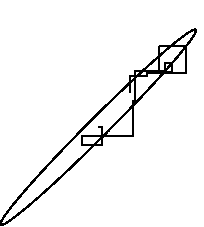
\includegraphics[width=\linewidth]{zoubin_figures/bvg-gibbs}
    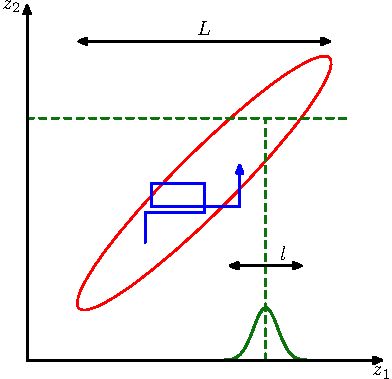
\includegraphics[width=\linewidth]{prmlfigs-pdf/Figure11_11}\\[-1cm]
    \begin{flushright}
    \Gray{\tiny Figure from PRML, Bishop (2006)}
    \end{flushright}
\end{minipage}

\vfill
\vfill
\Green{\bf Proof of validity:} \textbf{a)} check detailed balance for component update.\\
\textbf{b)} Metropolis--Hastings `proposals' $P(x_i|\bx_{j\neq i})\Rightarrow$ accept with prob. \rlap{$1$}\\
Apply a series of these operators. Don't need to check acceptance.

%%%%%%%%%%%%%%%%%%%%%%%%%%%%%%%%%%%%%%%%%%%%%%%%%%%%%%%%%%%%%%%%%%%%%%
\myfoilhead{Gibbs sampling}

\vfill
\Green{\bf Alternative explanation:}\\

Chain is currently at $\bx$\\

At equilibrium can assume $\bx \sim P(\bx)$\\

Consistent with $\bx_{j\neq i} \sim P(\bx_{j\neq i}), ~~ x_i \sim P(x_i\g \bx_{j\neq i})$\\

Pretend $x_i$ was never sampled and do it again.

\vfill
\vfill
\Gray{This view may be useful later for non-parametric applications}

% %%%%%%%%%%%%%%%%%%%%%%%%%%%%%%%%%%%%%%%%%%%%%%%%%%%%%%%%%%%%%%%%%%%%%%
% \myfoilhead{Is Gibbs sampling reversible?}
% 
% %%%%%%%%%%%%%%%%%%%%%%%%%%%%%%%%%%%%%%%%%%%%%%%%%%%%%%%%%%%%%%%%%%%%%%
% \myfoilhead{Ordered overrelaxation}

%%%%%%%%%%%%%%%%%%%%%%%%%%%%%%%%%%%%%%%%%%%%%%%%%%%%%%%%%%%%%%%%%%%%%%
\myfoilhead{\llap{``}Routine'' Gibbs sampling}

\vfill

{\bf Gibbs sampling benefits from few free choices and\\
\Green{\bf convenient features of conditional distributions}:}

\bigskip

\begin{itemize}
    \setlength{\itemsep}{5pt}
    \setlength{\parskip}{5pt}
    \setlength{\parsep}{0cm}
\item Conditionals with a few discrete settings can be \Green{explicitly normalized}:\\[-0.2in]

\hspace*{1cm}$\displaystyle P(x_i|\bx_{j\neq i}) \;\propto\; P(x_i,\bx_{j\neq i})$\\[0.2in]
\hspace*{1cm}$\displaystyle \phantom{P(x_i|\bx_{j\neq i})} \;=\; \frac{P(x_i,\bx_{j\neq i})}{\sum_{x'_i} P(x'_i,\bx_{j\neq i})\rlap{$~\la$ this sum is small and easy}}$\\

\item Continuous conditionals only univariate\\
    $\Rightarrow$ amenable to \Green{standard sampling methods}.
\end{itemize}

\vfill

{\tt WinBUGS} and {\tt OpenBUGS} sample graphical models using these tricks

% %%%%%%%%%%%%%%%%%%%%%%%%%%%%%%%%%%%%%%%%%%%%%%%%%%%%%%%%%%%%%%%%%%%%%%
% \mymessage{MCMC}%
% {-- tackles high-dimensional integrals\\
% -- good proposals may require ingenuity\\
% -- sometimes simple and routine\\
% -- but can be very slow}
% 
% %%%%%%%%%%%%%%%%%%%%%%%%%%%%%%%%%%%%%%%%%%%%%%%%%%%%%%%%%%%%%%%%%%%%%%
% \myfoilhead{Auxiliary variables}
% 
% \vspace*{2cm}
% 
% %Most MCMC methods are Metropolis--Hastings with some $Q(x';x)$\\
% 
% {\bf The point of MCMC is to marginalize out variables,\\
% but one can introduce more variables:}\\[-0.2in]
% \[
% \begin{split}
% \int f(x) P(x) \;\mathrm{d}x
% &= \int f(x) P(x,v) \;\mathrm{d}x\,\mathrm{d}v \\
% &\approx \frac{1}{S} \sum_{s=1}^S f(x^{(s)}), \quad x,v\sim P(x,v) \hphantom{\mbox{ \emph{rejecting} } v\neq v_0}
% \end{split}
% \]\\[-0.2in]
% 
% \vfill
% 
% \Green{\bf We might want to do this if}
% \begin{itemize}
%     \item $P(x,v)$ is easier to navigate
%     \item Example: $P(x|v)$ and $P(v|x)$ are simple
% \end{itemize}
% 
% \vfill
% 
% % or using $R(x,v)$ where $R(x|v\te v_0)=P(x)$
% % \[
% % \int f(x) P(x) \;\mathrm{d}x
% % \approx \frac{1}{S} \sum_{s=1}^S f(x^{(s)}), \quad (x,v)\sim R(x,v) \mbox{ \emph{reject} if } v\neq v_0
% % \]
% 
% %\vfill
% 
% %\Green{\textbf{Auxiliary variables}} are extra work but can help navigation %\\
% %E.g.: $v=$``temperature'', $R(x|v>v_0)$ much more diffuse than $P(x)$

%%%%%%%%%%%%%%%%%%%%%%%%%%%%%%%%%%%%%%%%%%%%%%%%%%%%%%%%%%%%%%%%%%%%%%
\myfoilhead{Summary so far}

\vfill

\begin{minipage}{0.05\linewidth}
    ~
\end{minipage}
\begin{minipage}{0.9\linewidth}
\begin{itemize}
    \setlength{\itemsep}{5pt}
    \setlength{\parskip}{5pt}
    \setlength{\parsep}{0cm}
    %\setlength{\itemindent}{0em}
    %\setlength{\listparindent}{0em}
    %\setlength{\leftmargini}{0em}
    %\setlength{\leftmargin}{0em}
    \item We need approximate methods to solve sums/integrals
    \item Monte Carlo does not explicitly depend on dimension,\\
        although simple methods work only in low dimensions
    \item \Green{Markov chain Monte Carlo (MCMC) can make local moves.}\\
        By assuming less, it's more applicable to higher dimensions
    \item simple computations $\Rightarrow$ ``easy'' to implement\\
        (harder to diagnose).
\end{itemize}
\end{minipage}

\vfill
\vfill

\Green{\bf How do we use these MCMC samples?}

%%%%%%%%%%%%%%%%%%%%%%%%%%%%%%%%%%%%%%%%%%%%%%%%%%%%%%%%%%%%%%%%%%%%%%
\newpage

\vspace*\fill

\Gray{
\begin{tabular*}{\textwidth}{l}
\toprule\\
{\bf \Huge End of Lecture 1} \\[0.4in]
\bottomrule
\end{tabular*}}

\vfill
\vfill

%%%%%%%%%%%%%%%%%%%%%%%%%%%%%%%%%%%%%%%%%%%%%%%%%%%%%%%%%%%%%%%%%%%%%%
\myfoilhead{Quick review}

\vspace*{1cm}

\Green{\bf Construct a biased random walk that explores a target dist.}

\vspace*{1cm}

\hspace*{-1cm}
\begin{minipage}{0.5\linewidth}
\centerline{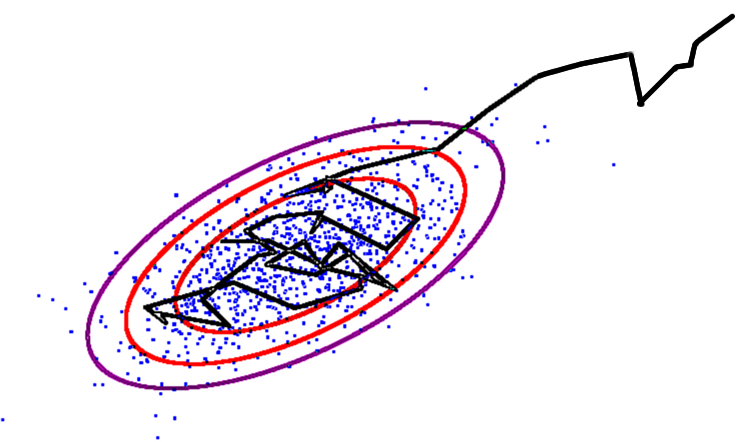
\includegraphics[scale=1.3]{mcmc2}}
\vspace*{1cm}
\end{minipage}
\begin{minipage}{0.6\linewidth}
    Markov steps, $x^{(s)}\sim T\big(x^{(s)}\la x^{(s-1)}\big)$

\vspace*{1cm}

\Red{MCMC gives approximate,\\correlated samples}

\vspace*{1cm}

$\displaystyle \ave{P}{f} \approx \frac{1}{S} \sum_{s=1}^S f(x^{(s)})$
\end{minipage}

\vfill

\Green{\bf Example transitions:}

\bigskip

\textbf{Metropolis--Hastings:} $\displaystyle T(x'\la x) = Q(x'; x) \, \min\kern-3pt\left( 1,\;
\frac{P(x')\,Q(x;x')}{P(x)\,Q(x';x)}\right)$

\bigskip
\bigskip

\textbf{Gibbs sampling:} $\displaystyle T_i(\bx'\la \bx) = P(x'_i\g \bx_{j\neq i}) \, \delta( \bx'_{j\neq i} - \bx_{j\neq i})$



%%%%%%%%%%%%%%%%%%%%%%%%%%%%%%%%%%%%%%%%%%%%%%%%%%%%%%%%%%%%%%%%%%%%%%
\myfoilhead{How should we run MCMC?}

\vfill

\begin{minipage}{0.05\linewidth}
    ~
\end{minipage}
\begin{minipage}{0.9\linewidth}
\begin{itemize}
    \setlength{\itemsep}{10pt}
    \setlength{\parskip}{5pt}
    \setlength{\parsep}{0cm}
    %\setlength{\itemindent}{0em}
    %\setlength{\listparindent}{0em}
    %\setlength{\leftmargini}{0em}
    %\setlength{\leftmargin}{0em}
    \item The samples aren't independent. Should we \Green{\bf thin},\\
        only keep every $K$th sample?
    \item Arbitrary initialization means starting iterations are bad.\\
        Should we discard a \Green{\bf ``burn-in'' period}?
    \item Maybe we should perform \Green{\bf multiple runs?}
    \item How do we know if we have run for \Green{\bf long enough?}
\end{itemize}
\end{minipage}
\vspace*{-2.5cm}
\vfill
\hspace*{16cm}{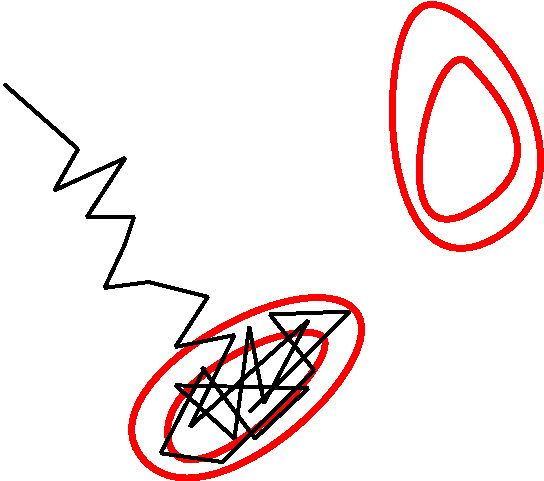
\includegraphics[scale=1]{burn_in_and_mix}\hspace*{3cm}}
\vspace*{-0.7cm}

%%%%%%%%%%%%%%%%%%%%%%%%%%%%%%%%%%%%%%%%%%%%%%%%%%%%%%%%%%%%%%%%%%%%%%
\myfoilhead{Forming estimates}

\vfill

Approximately independent samples can be obtained by \emph{thinning}.\\
However, \Green{\bf all the samples can be used.}\\

\Green{\bf Use the simple Monte Carlo estimator on MCMC samples.} It is:\\
\hspace*{3cm}--- consistent\\
\hspace*{3cm}--- unbiased if the chain has ``burned in''

\vfill
\Green{\bf The correct motivation to thin:} if computing $f(\bx^{(s)})$ is expensive
\vfill

%%%%%%%%%%%%%%%%%%%%%%%%%%%%%%%%%%%%%%%%%%%%%%%%%%%%%%%%%%%%%%%%%%%%%%
\myfoilhead{Empirical diagnostics}

\vspace*{1cm}

\centerline{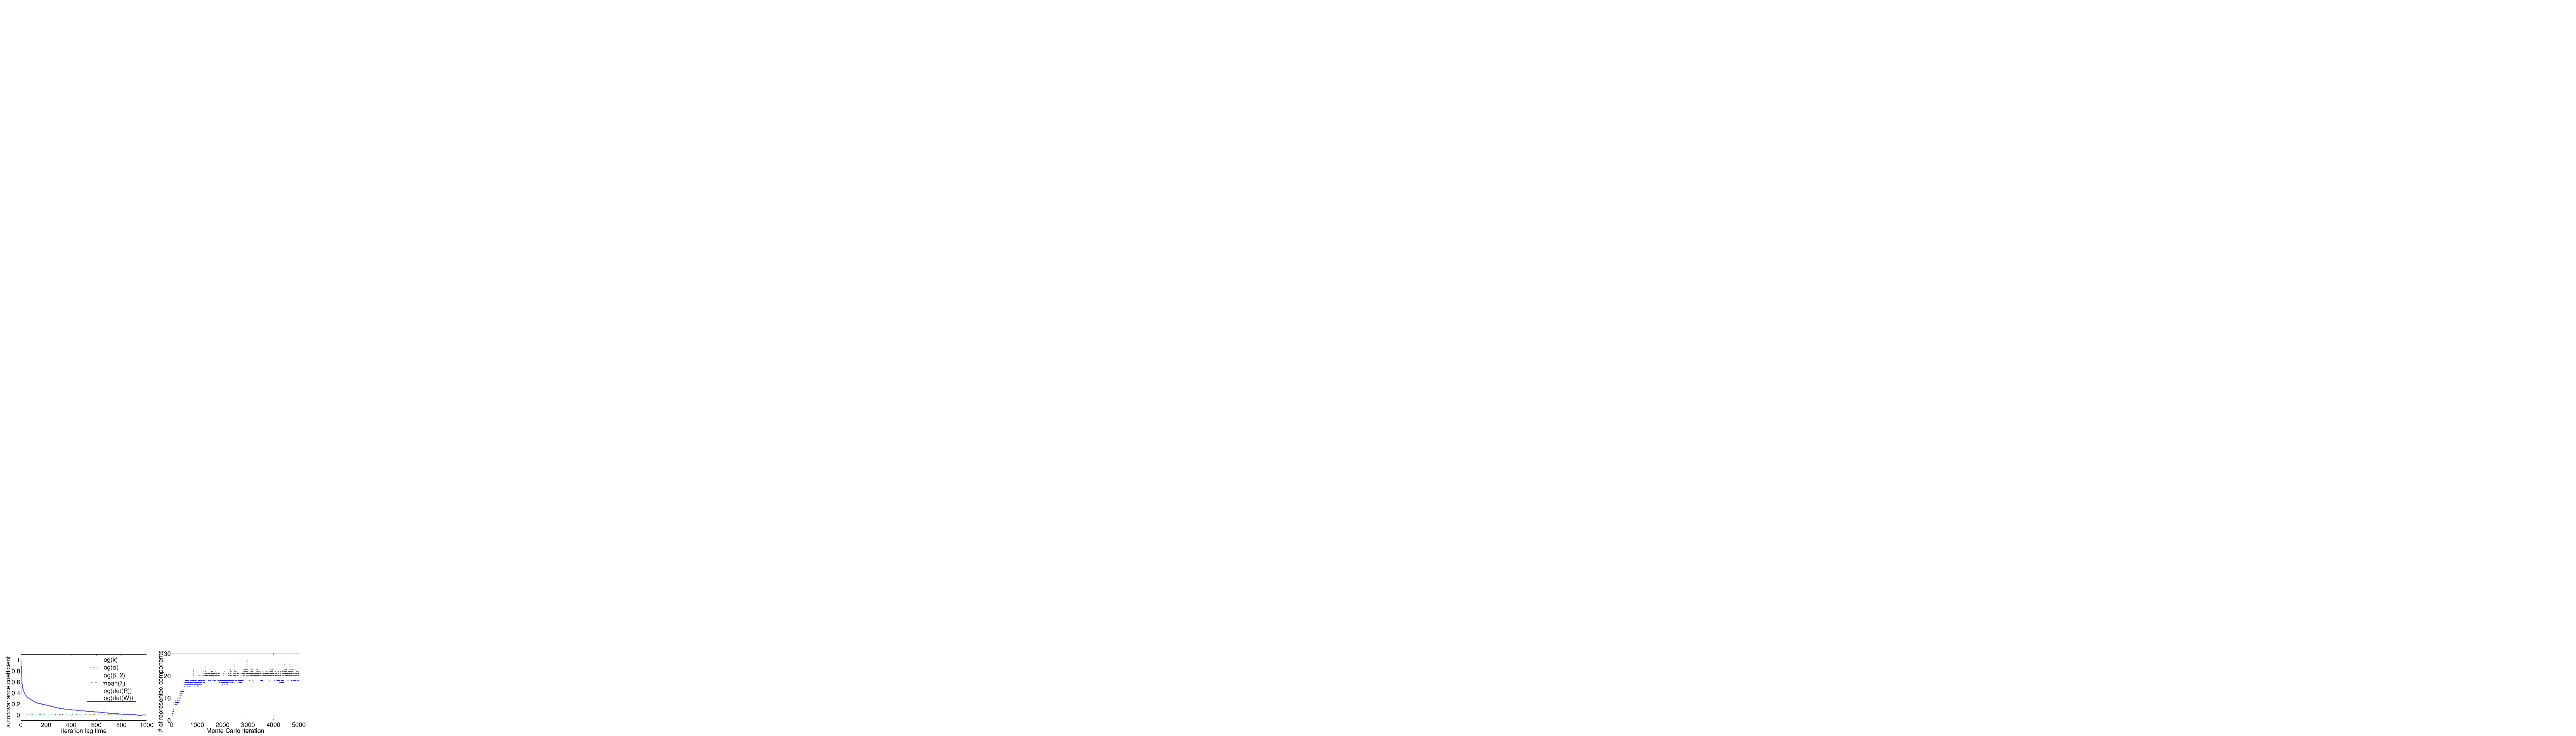
\includegraphics[width=\linewidth]{rasmussen2000b}}
\begin{flushright}
    \Gray{Rasmussen (2000)}
\end{flushright}

\vfill

{\Green{\bf Recommendations}\\[-0.2in]

\small \textbf{For diagnostics:}\\
Standard software packages like \texttt{R-CODA}\\[-0.2in]

\textbf{For opinion on thinning, multiple runs, burn in, etc.}\\
Practical Markov chain Monte Carlo\\[-0.1in]
Charles J. Geyer, \textit{Statistical Science}. 7(4):473--483, 1992.\\[-0.1in]
\texttt{http://www.jstor.org/stable/2246094}}

%%%%%%%%%%%%%%%%%%%%%%%%%%%%%%%%%%%%%%%%%%%%%%%%%%%%%%%%%%%%%%%%%%%%%%
\myfoilhead{Consistency checks}

\vspace*{3cm}

\Green{\large \bf Do I get the right answer on tiny versions\\[0.1in] of my problem?}

\vspace*{3cm}

\Green{\large \bf Can I make good inferences about synthetic data\\[0.1in]
drawn from my model?}

\vspace*{2cm}

\bigskip

\textbf{Getting it right:} joint distribution tests of posterior simulators,\\
John Geweke, \textit{JASA}, 99(467):799--804, 2004.

\vfill
\begin{flushright}
    \Gray{\tiny [next: using the samples]}
\end{flushright}
% %%%%%%%%%%%%%%%%%%%%%%%%%%%%%%%%%%%%%%%%%%%%%%%%%%%%%%%%%%%%%%%%%%%%%%
% \myfoilhead{Three worries}
% 
% \vspace*{1.5cm}
% 
% \Green{\bf Mixing:}\\[0.2in]
% \myindent{Efficient burn-in and mode\\exploration can be a problem}
% 
% \vspace*{-3.5cm}
% 
% \hfill 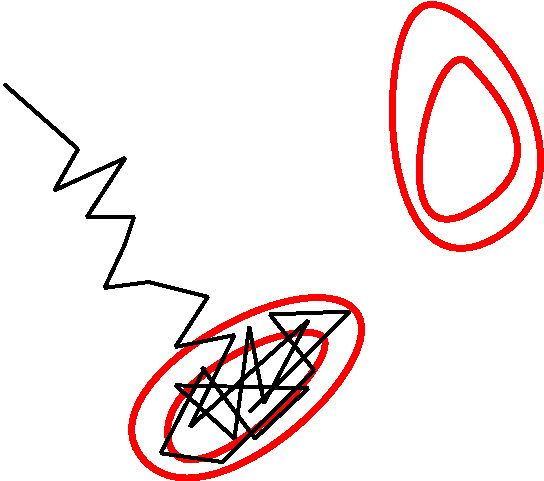
\includegraphics[scale=0.75]{burn_in_and_mix}\hspace*{3cm}
% 
% \vfill
% 
% \Green{\bf Will the standard estimator work?}\\[0.2in]
% \myindent{e.g.\ need many samples from a\\ distribution to estimate its tail}\\
% 
% \vspace*{-2.5cm}
% 
% \hfill 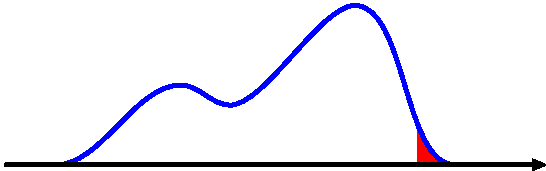
\includegraphics{rejection/rejection3}
% 
% \vspace*{2.5cm}
% 
% \vfill
% 
% \Green{\bf Normalizing constants}\\[0.2in]
% \myindent{$\displaystyle p(x)=\frac{\tilde{p}(x)}{\Z}$, MCMC doesn't need $\Z$\dots or find it either}

% %%%%%%%%%%%%%%%%%%%%%%%%%%%%%%%%%%%%%%%%%%%%%%%%%%%%%%%%%%%%%%%%%%%%%%
% \myfoilhead{A common concern}
% 
% \vspace*{2.5cm}
% 
% \Green{\bf Mixing:} Efficient burn-in and mode exploration can be a problem
% 
% \vfill
% 
% \centerline{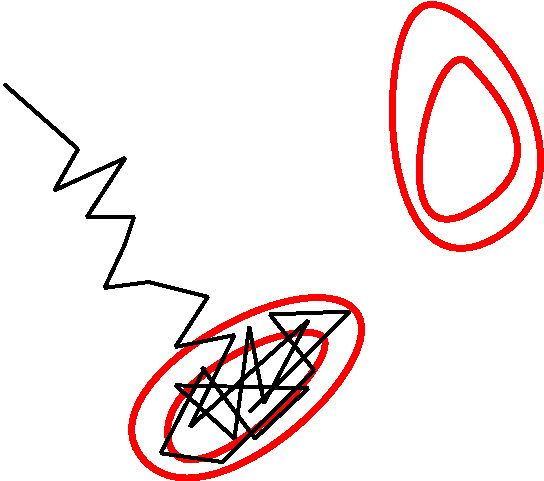
\includegraphics[scale=1.5]{burn_in_and_mix}\hspace*{3cm}}

%\Green{\bf Normalizing constants}\\[0.2in]
%\myindent{$\displaystyle p(x)=\frac{\tilde{p}(x)}{\Z}$, MCMC doesn't need $\Z$\dots or find it either}

%%%%%%%%%%%%%%%%%%%%%%%%%%%%%%%%%%%%%%%%%%%%%%%%%%%%%%%%%%%%%%%%%%%%%%
\myfoilhead{Making good use of samples}

\vspace*{2cm}

\Green{\bf Is the standard estimator too noisy?}\\[0.2in]
\myindent{e.g.\ need many samples from a\\ distribution to estimate its tail}\\

\vspace*{-2.5cm}

\hfill 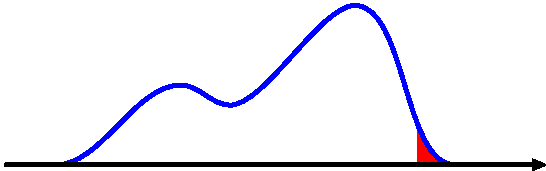
\includegraphics{rejection/rejection3}

\vspace*{0.5cm}
\myindent{We can often do \emph{some} analytic calculations}

\vfill


%%%%%%%%%%%%%%%%%%%%%%%%%%%%%%%%%%%%%%%%%%%%%%%%%%%%%%%%%%%%%%%%%%%%%%
\myfoilhead{Finding $P(x_i\te 1)$}

\vfill

\Green{{\bf Method 1:}} fraction of time $x_i\te 1$
\[
P(x_i\te 1) = \sum_{x_i} \I(x_i\te 1) P(x_i) \approx \frac{1}{S} \sum_{s=1}^S \I(x_i^{(s)}), \quad x_i^{(s)}\sim P(x_i)
\]

\vfill

\Green{{\bf Method 2:}} average of $P(x_i\te 1|\bx_{\backslash i})$
\[
\begin{split}
P(x_i\te 1) &= \sum_{\bx_{\backslash i}} P(x_i\te 1|\bx_{\backslash i}) P(\bx_{\backslash i})\\
    &\approx \frac{1}{S} \sum_{s=1}^S P(x_i=1|\bx_{\backslash i}^{(s)}), \quad\bx_{\backslash i}^{(s)}\sim P(\bx_{\backslash i})
\end{split}
\]

\vfill
{\textbf{Example of ``Rao-Blackwellization''.  See also ``waste recycling''.}}

%%%%%%%%%%%%%%%%%%%%%%%%%%%%%%%%%%%%%%%%%%%%%%%%%%%%%%%%%%%%%%%%%%%%%%
\myfoilhead{Processing samples}

\vspace*{1.5cm}

\Green{\bf This is easy}\\[-0.4in]
\[
I = \sum_{\bx} f(x_i) P(\bx) \approx \frac{1}{S} \sum_{s=1}^S f(x_i^{(s)}), \quad \bx^{(s)}\sim P(\bx)
\]

\vfill

\Green{\bf But this might be better}\\[-0.2in]
\[
\begin{split}
I &= \sum_{\bx} f(x_i) P(x_i|\bx_{\backslash i}) P(\bx_{\backslash i})
  = \sum_{\bx_{\backslash i}} \bigg(\sum_{x_i} f(x_i) P(x_i|\bx_{\backslash i})\bigg) P(\bx_{\backslash i})\\
  &\approx \frac{1}{S} \sum_{s=1}^S \bigg(\sum_{x_i} f(x_i) P(x_i|\bx_{\backslash i}^{(s)})\bigg), \quad\bx_{\backslash i}^{(s)}\sim P(\bx_{\backslash i}) \end{split}
\]

\vfill
\textbf{A more general form of ``Rao-Blackwellization''.}

%%%%%%%%%%%%%%%%%%%%%%%%%%%%%%%%%%%%%%%%%%%%%%%%%%%%%%%%%%%%%%%%%%%%%%
\myfoilhead{Summary so far}

\vfill

\begin{itemize}
    \setlength{\itemsep}{10pt}
    \setlength{\parskip}{10pt}
    \setlength{\parsep}{0cm}

\item MCMC algorithms are general and often easy to implement

\item Running them \emph{is} a bit messy\dots\\
    \dots but there are some established procedures.

\item Given the samples there might be a choice of estimators

\end{itemize}

\vfill
\vfill

\Green{\bf Next question}:\\
Is MCMC research all about finding a good $Q(\bx)$?

%%%%%%%%%%%%%%%%%%%%%%%%%%%%%%%%%%%%%%%%%%%%%%%%%%%%%%%%%%%%%%%%%%%%%%
\myfoilhead{Auxiliary variables}

\vspace*{2cm}

%Most MCMC methods are Metropolis--Hastings with some $Q(x';x)$\\

{\bf The point of MCMC is to marginalize out variables,\\
but one can introduce more variables:}\\[-0.2in]
\[
\begin{split}
\int f(x) P(x) \;\mathrm{d}x
&= \int f(x) P(x,v) \;\mathrm{d}x\,\mathrm{d}v \\
&\approx \frac{1}{S} \sum_{s=1}^S f(x^{(s)}), \quad x,v\sim P(x,v) \hphantom{\mbox{ \emph{rejecting} } v\neq v_0}
\end{split}
\]\\[-0.2in]

\vfill

\Green{\bf We might want to do this if}
\begin{itemize}
    \item $P(x|v)$ and $P(v|x)$ are simple
    \item $P(x,v)$ is otherwise easier to navigate
\end{itemize}

\vfill

% or using $R(x,v)$ where $R(x|v\te v_0)=P(x)$
% \[
% \int f(x) P(x) \;\mathrm{d}x
% \approx \frac{1}{S} \sum_{s=1}^S f(x^{(s)}), \quad (x,v)\sim R(x,v) \mbox{ \emph{reject} if } v\neq v_0
% \]

%\vfill

%\Green{\textbf{Auxiliary variables}} are extra work but can help navigation %\\
%E.g.: $v=$``temperature'', $R(x|v>v_0)$ much more diffuse than $P(x)$

%%%%%%%%%%%%%%%%%%%%%%%%%%%%%%%%%%%%%%%%%%%%%%%%%%%%%%%%%%%%%%%%%%%%%%
\myfoilhead{Swendsen--Wang (1987)}

\vfill

Seminal algorithm using auxiliary variables\\

Edwards and Sokal (1988) identified and generalized the\\
``Fortuin-Kasteleyn-Swendsen-Wang'' auxiliary variable joint\\
distribution that underlies the algorithm.

\vfill

\hspace*{-0.9cm}
\includegraphics[scale=0.7]{sw_pics/sw32}
\includegraphics[scale=0.7]{sw_pics/sw33}
%\includegraphics[scale=0.5]{sw_pics/sw34}
\includegraphics[scale=0.7]{sw_pics/sw35}

\vspace*{-0.5cm}

%%%%%%%%%%%%%%%%%%%%%%%%%%%%%%%%%%%%%%%%%%%%%%%%%%%%%%%%%%%%%%%%%%%%%%
\myfoilhead{Slice sampling idea}

\vspace*{1.5cm}

\Green{\bf Sample point uniformly under curve $\tilde{P}(x)\propto P(x)$}

\vfill

\centerline{\includegraphics[scale=2.5]{slice/slice0}}

\vfill

%\Green{\bf Height $u$ is an auxiliary variable:}\\[0.1in]
\hspace*{2cm} $p(u|x)=\mbox{Uniform}[0,\tilde{P}(x)]$\\[0.5in]
\hspace*{2cm} $p(x|u)\propto \begin{cases} 1 & \tilde{P}(x)\ge u\\
                                           0 & \mbox{otherwise}
                                       \end{cases} = \mbox{``Uniform on the slice''}$



%%%%%%%%%%%%%%%%%%%%%%%%%%%%%%%%%%%%%%%%%%%%%%%%%%%%%%%%%%%%%%%%%%%%%%
\myfoilhead{Slice sampling}

\vspace*{1.5cm}

\Green{\bf Unimodal conditionals}\\

\includegraphics[scale=1.4]{slice/slice1}\hfill%
\includegraphics[scale=1.4]{slice/slice2}\hfill%
\includegraphics[scale=1.4]{slice/slice3}

\vfill

\begin{itemize}
    \setlength{\itemsep}{5pt}
    \setlength{\parskip}{5pt}
    \setlength{\parsep}{0cm}
    \item bracket slice
    \item sample uniformly within bracket
    \item shrink bracket if $\tilde{P}(x)<u$ (off slice)
    \item accept first point on the slice
\end{itemize}

\vfill

%%%%%%%%%%%%%%%%%%%%%%%%%%%%%%%%%%%%%%%%%%%%%%%%%%%%%%%%%%%%%%%%%%%%%%
\myfoilhead{Slice sampling}

\vspace*{1.5cm}

\Green{\bf Multimodal conditionals}\\

\centerline{\includegraphics[scale=2.5]{slice/slice4}}

\vfill

\begin{itemize}
    \setlength{\itemsep}{5pt}
    \setlength{\parskip}{5pt}
    \setlength{\parsep}{0cm}
    \item place bracket randomly around point
    \item linearly step out until bracket ends are off slice
    \item sample on bracket, shrinking as before
\end{itemize}

\Green{\bf Satisfies detailed balance}, leaves $p(x|u)$ invariant

%%%%%%%%%%%%%%%%%%%%%%%%%%%%%%%%%%%%%%%%%%%%%%%%%%%%%%%%%%%%%%%%%%%%%%
\myfoilhead{Slice sampling}

\vfill

%Before today I have given a 2 hour talk on just slice sampling

\Green{\bf Advantages of slice-sampling:}
\begin{itemize}
    \setlength{\itemsep}{5pt}
    \setlength{\parskip}{5pt}
    \setlength{\parsep}{0cm}
\item Easy --- only require $\tilde{P}(x)\propto P(x)$ pointwise
    \item No rejections
    \item Step-size parameters less important than Metropolis
%    \item Linear bracketing one of several operators on slice
%    \item Also provides frameworks for:
%    \begin{itemize}
%        \item adaptation
%        \item random walk reduction
%    \end{itemize}
\end{itemize}

\vfill
\vfill
More advanced versions of slice sampling have been developed.\\
Neal (2003) contains \emph{many} ideas.

%%%%%%%%%%%%%%%%%%%%%%%%%%%%%%%%%%%%%%%%%%%%%%%%%%%%%%%%%%%%%%%%%%%%%%
\myfoilhead{Hamiltonian dynamics}

\vfill

\Green{\bf Construct a landscape} with gravitational potential energy, E(x):\\[0.2in]
\hspace*{2cm} $P(x)\propto e^{-E(x)}, \qquad E(x)=-\log P^*(x)$\\

% Simple $\N(x,\sigma^2)$ Metropolis--Hastings proposals $\rightarrow$ slow diffusion\\
% A dynamical system can give persistent motion across the landscape\\

\Green{\bf Introduce velocity} $v$ carrying kinetic energy $K(v)=v^\top v/2$\\

\vfill

\Green{\bf Some physics:}
\begin{itemize}
    \item Total energy or Hamiltonian, $H=E(x)+K(v)$ 
    \item Frictionless ball rolling $(x,v)\ra (x',v')$ satisfies $H(x',v')=H(x,v)$
    \item Ideal Hamiltonian dynamics are time reversible:
    \begin{itemize}
        \item reverse $v$ and the ball will return to its start point
    \end{itemize}
\end{itemize}

%%%%%%%%%%%%%%%%%%%%%%%%%%%%%%%%%%%%%%%%%%%%%%%%%%%%%%%%%%%%%%%%%%%%
\myfoilhead{Hamiltonian Monte Carlo}

\vfill

\Green{\bf Define a joint distribution:}
\begin{itemize}
    \setlength{\itemsep}{5pt}
    \setlength{\parskip}{5pt}
    \setlength{\parsep}{0cm}
    \item $P(x,v) \propto e^{-E(x)}e^{-K(v)} = e^{-E(x)-K(v)} = e^{-H(x,v)}$
    \item Velocity is independent of position and Gaussian distributed
\end{itemize}

\vfill

\Green{\bf Markov chain operators}
\begin{itemize}
    \setlength{\itemsep}{5pt}
    \setlength{\parskip}{5pt}
    \setlength{\parsep}{0cm}
    \item Gibbs sample velocity
    \item Simulate Hamiltonian dynamics then flip sign of velocity
    \begin{itemize}
        \item Hamiltonian `proposal' is deterministic and reversible\\$q(x',v';x,v)=q(x,v;x',v')=1$
        \item Conservation of energy means $P(x,v)=P(x',v')$
        \item Metropolis acceptance probability is 1
    \end{itemize}
\end{itemize}

\vfill

\Green{\bf Except we can't simulate Hamiltonian dynamics exactly}


%%%%%%%%%%%%%%%%%%%%%%%%%%%%%%%%%%%%%%%%%%%%%%%%%%%%%%%%%%%%%%%%%%%%
\myfoilhead{Leap-frog dynamics}

\vfill

\Green{\bf a discrete approximation to Hamiltonian dynamics:}
\begin{eqnarray*}
    v_i(t+{\textstyle \frac{\epsilon}{2}}) & = & v_i(t) -
\frac{\epsilon}{2}\ \frac{\partial E(x(t))}{\partial x_i}\\
x_i(t+\epsilon) & = & x_i(t) +
\epsilon\kern3pt v_i(t+{\textstyle \frac{\epsilon}{2}})\\
p_i(t+\epsilon) & = & v_i(t+{\textstyle \frac{\epsilon}{2}}) -
\frac{\epsilon}{2}\ \frac{\partial E(x(t+\epsilon))}{\partial x_i}
\end{eqnarray*}

\begin{itemize}
    \item $H$ is not conserved
    \item dynamics are still deterministic and reversible
    \item Acceptance probability becomes $\min[1,\exp(H(v,x)-H(v',x'))]$
\end{itemize}

\vfill
\vfill

%%%%%%%%%%%%%%%%%%%%%%%%%%%%%%%%%%%%%%%%%%%%%%%%%%%%%%%%%%%%%%%%%%%%
\myfoilhead{Hamiltonian Monte Carlo}

\vfill

\begin{minipage}{0.6\linewidth}

    \Green{\bf The algorithm:}
\begin{itemize}
    \item Gibbs sample velocity $\sim \N(0,\,\I)$
    \item Simulate Leapfrog dynamics for $L$ steps
    \item Accept new position with probability\\
          $\min[1,\exp(H(v,x)-H(v',x'))]$
\end{itemize}

\bigskip

\end{minipage}
\begin{minipage}{0.39\linewidth}
    \includegraphics[width=\linewidth]{zoubin_figures/bvg-hybrid}
\end{minipage}


\vfill

The original name is \Green{\bf Hybrid Monte Carlo}, with reference
to the ``hybrid'' dynamical simulation method on which it was based.
%%%%%%%%%%%%%%%%%%%%%%%%%%%%%%%%%%%%%%%%%%%%%%%%%%%%%%%%%%%%%%%%%%%%%%
% \myfoilhead{MCMC's main problem}
% 
% \vfill
% 
% \Green{\bf Mixing:}\\[0.2in]
% \myindent{Efficient burn-in and\\mode exploration}
% 
% \vspace*{-3.5cm}
% 
% \hfill \includegraphics[scale=0.75]{burn_in_and_mix}\hspace*{5cm}
% 
% \vfill
% \vfill
% %\vfill
% %\vfill
% %\hfill {\large \sc [The End]}

%%%%%%%%%%%%%%%%%%%%%%%%%%%%%%%%%%%%%%%%%%%%%%%%%%%%%%%%%%%%%%%%%%%%%%
\myfoilhead{Summary of auxiliary variables}

\vfill

--- Swendsen--Wang\\
--- Slice sampling\\
--- Hamiltonian (Hybrid) Monte Carlo

\vfill

A fair amount of my research (not covered in this tutorial) has been finding the
right auxiliary representation on which to run standard MCMC updates.\\

{\bf Example benefits:}

\bigskip
Population methods to give better mixing and exploit parallel hardware

\bigskip

Being robust to bad random number generators

\bigskip
Removing step-size parameters when slice sample doesn't really apply



%%%%%%%%%%%%%%%%%%%%%%%%%%%%%%%%%%%%%%%%%%%%%%%%%%%%%%%%%%%%%%%%%%%%%%
\myfoilhead{Finding normalizers is hard}

\vspace*{1.5cm}

{\bf \Green{Prior sampling:} like finding fraction of needles in a hay-stack}
\[
\begin{split}
P(\D|\M) &= \int P(\D|\theta,\M) P(\theta|\M)\;\mathrm{d}\theta\\
&= \frac{1}{S} \sum_{s=1}^S P(\D|\theta^{(s)},\M), \quad \theta^{(s)}\sim P(\theta|\M)\\
&\phantom{= }\mbox{\bf \dots usually has huge variance}
\end{split}
\]

\vspace*{1cm}

\Green{\bf Similarly for undirected graphs:}
\[
    P(\bx) = \frac{P^*(\bx)}{\Z}, \qquad \Z = \sum_{\bx} P^*(\bx)
\]
I will use this as an easy-to-illustrate case-study

%%%%%%%%%%%%%%%%%%%%%%%%%%%%%%%%%%%%%%%%%%%%%%%%%%%%%%%%%%%%%%%%%%%%%%
\myfoilhead{Benchmark experiment}

\vfill

\hspace*{\fill}
\includegraphics[scale=0.65]{icml_figs/train_samples}
\hspace*{\fill}
\includegraphics[scale=0.7]{icml_figs/CD25_500_samples}
\hspace*{\fill}
\includegraphics[scale=0.58]{icml_figs/MoB100}
\hspace*{\fill}
\bigskip

\hspace*{2.0cm}\hbox{Training set}
\hspace*{3.5cm}\hbox{RBM samples}
\hspace*{3.0cm}\hbox{MoB samples}

\vfill
\textbf{RBM setup:}\\
\hspace*{2cm}--- $28\times 28 = 784$ binary visible variables\\
\hspace*{2cm}--- $500$ binary hidden variables

\bigskip

\textbf{Goal:} Compare $P(\bx)$ on test set, ($P_\text{RBM}(\bx)=P^*(\bx)/\Z$)

%%%%%%%%%%%%%%%%%%%%%%%%%%%%%%%%%%%%%%%%%%%%%%%%%%%%%%%%%%%%%%%%%%%%%%
\myfoilhead{Simple Importance Sampling}

\vspace*{1.5cm}

$\displaystyle \Z
%~=~
%\sum_\bx P^*(\bx)
~=~
\sum_\bx \frac{P^*(\bx)}{Q(\bx)}\,Q(\bx)
~\approx~
\frac{1}{S} \sum_{s=1}^S \frac{P^*(\bx\sth)}{Q(\bx)},\quad {\small \bx\sth\sim Q(\bx)}
$

\vfill

$\bx^{(1)}\!=\,$\myvcenter{\includegraphics[width=0.1\linewidth]{hundred/figure0}},~~~
$\bx^{(2)}\!=\,$\myvcenter{\includegraphics[width=0.1\linewidth]{hundred/figure1}},~~~
$\bx^{(3)}\!=\,$\myvcenter{\includegraphics[width=0.1\linewidth]{hundred/figure2}},\\[0.3in]
$\bx^{(4)}\!=\,$\myvcenter{\includegraphics[width=0.1\linewidth]{hundred/figure3}},~~~
$\bx^{(5)}\!=\,$\myvcenter{\includegraphics[width=0.1\linewidth]{hundred/figure4}},~~~
$\bx^{(6)}\!=\,$\myvcenter{\includegraphics[width=0.1\linewidth]{hundred/figure5}},\dots

\vfill
\Gray{$\displaystyle \Z
~=~
2^D \sum_{\bx} \frac{1}{2^D} P^*(\bx)
~\approx~
\frac{2^D}{S} \sum_{s=1}^S P^*(\bx\sth),\quad {\small \bx\sth\sim \text{Uniform}}$}

%%%%%%%%%%%%%%%%%%%%%%%%%%%%%%%%%%%%%%%%%%%%%%%%%%%%%%%%%%%%%%%%%%%%%%
\myfoilhead{``Posterior'' Sampling}

\vfill

Sample from $\displaystyle P(\bx) = \frac{P^*(\bx)}{\Z}$,~~~~~
\Gray{\small $\displaystyle \left[\text{or~}P(\theta|\D) = \frac{P(\D|\theta)P(\theta)}{P(\D)}\right]$}

\vfill

$\bx^{(1)}\!=\,$\myvcenter{\includegraphics[width=0.1\linewidth]{posterior/sample01}},~~~
$\bx^{(2)}\!=\,$\myvcenter{\includegraphics[width=0.1\linewidth]{posterior/sample02}},~~~
$\bx^{(3)}\!=\,$\myvcenter{\includegraphics[width=0.1\linewidth]{posterior/sample03}},\\[0.3in]
$\bx^{(4)}\!=\,$\myvcenter{\includegraphics[width=0.1\linewidth]{posterior/sample04}},~~~
$\bx^{(5)}\!=\,$\myvcenter{\includegraphics[width=0.1\linewidth]{posterior/sample05}},~~~
$\bx^{(6)}\!=\,$\myvcenter{\includegraphics[width=0.1\linewidth]{posterior/sample06}},\dots

\vfill

$\displaystyle \Red{\Z = \sum_{\bx} P^*(\bx)}$
\hspace*\fill
$\displaystyle \Z \text{~``$\approx$''~} \frac{1}{S} \sum_{s=1}^S \frac{P^*(\bx)}{P(\bx)} = \Z$


%%%%%%%%%%%%%%%%%%%%%%%%%%%%%%%%%%%%%%%%%%%%%%%%%%%%%%%%%%%%%%%%%%%%%%
\myfoilhead{Finding a Volume}

\vfill
\vfill

\hspace*{0.5cm}\myvcenter{\scalebox{2}{$\rightarrow$}} $\bx$\\
\myvcenter{\scalebox{2}{$\downarrow$}}\\[0.6cm] $P^*(\bx)$

\vspace*{-4.5cm}
\centerline{\includegraphics[width=0.8\linewidth]{lake/figure207}}

\vfill
\Gray{Lake analogy and figure from MacKay textbook (2003)}

%%%%%%%%%%%%%%%%%%%%%%%%%%%%%%%%%%%%%%%%%%%%%%%%%%%%%%%%%%%%%%%%%%%%%%
\myfoilhead{Annealing / Tempering}

\begin{center}
\[
%\mbox{e.g.\ }P(\bx;\beta) = \frac{1}{\Z(\beta)} \sum_\bh P(\bx,\bh|\theta)^\beta \, \pi(\bx)^{(1-\beta)}
% Lie to simplify:
\mbox{e.g.\ }P(\bx;\beta) ~\propto~ P^*(\bx)^\beta \, \pi(\bx)^{(1-\beta)}
\]

\vspace{-2cm}

\parbox[b]{0.125\textwidth}{\begin{center}\includegraphics[scale=0.8]{tempplots2/beta0}\\\scalebox{0.9}{\small $\beta=0$}\end{center}}
\hfill
\parbox[b]{0.125\textwidth}{\begin{center}\includegraphics[scale=0.8]{tempplots2/beta1}\\\scalebox{0.9}{\small $\beta=0.01$}\end{center}}
\hfill
\parbox[b]{0.125\textwidth}{\begin{center}\includegraphics[scale=0.8]{tempplots2/beta2}\\\scalebox{0.9}{\small $\beta=0.1$}\end{center}}
\hfill
\parbox[b]{0.125\textwidth}{\begin{center}\includegraphics[scale=0.8]{tempplots2/beta3}\\\scalebox{0.9}{\small $\beta=0.25$}\end{center}}
\hfill
\parbox[b]{0.125\textwidth}{\begin{center}\includegraphics[scale=0.8]{tempplots2/beta4}\\\scalebox{0.9}{\small $\beta=0.5$}\end{center}}
\hfill
\parbox[b]{0.125\textwidth}{\begin{center}\includegraphics[scale=0.8]{tempplots2/beta5}\\\scalebox{0.9}{\small $\beta=1$}\end{center}}
\end{center}

\vfill

\includegraphics[width=0.24\linewidth]{icml_figs/baserate_samples}
\includegraphics[width=0.24\linewidth]{icml_figs/CD25_05}
\includegraphics[width=0.24\linewidth]{icml_figs/CD25_95}
\includegraphics[width=0.24\linewidth]{icml_figs/CD25_10}


\vfill
%    $\displaystyle \frac{\Z(1)}{\Z(0)} =
%        \frac{\Z(\beta_1)}{\Z(0)}\cdot
%        \frac{\Z(\beta_2)}{\Z(\beta_1)}\cdot
%        \frac{\Z(\beta_3)}{\Z(\beta_2)}\cdot
%        \frac{\Z(\beta_4)}{\Z(\beta_3)}\cdot
%        \frac{\Z(1)}{\Z(\beta_4)}$

$1/\beta \,= $ ``temperature''

%%%%%%%%%%%%%%%%%%%%%%%%%%%%%%%%%%%%%%%%%%%%%%%%%%%%%%%%%%%%%%%%%%%%%%
\myfoilhead{Using other distributions}

\vspace*{1.5cm}

\Green{\bf \emph{Chain} between posterior and prior:}

\vspace*{-1cm}

\begin{center}
\[
\mbox{e.g.\ }P(\theta;\beta) = \frac{1}{\Z(\beta)} P(\D|\theta)^\beta P(\theta)
\]

\vspace{-2cm}

\parbox[b]{0.125\textwidth}{\begin{center}\includegraphics[scale=0.8]{tempplots2/beta0}\\\small $\beta=0$\end{center}}
\hfill
\parbox[b]{0.125\textwidth}{\begin{center}\includegraphics[scale=0.8]{tempplots2/beta1}\\\small $\beta=0.01$\end{center}}
\hfill
\parbox[b]{0.125\textwidth}{\begin{center}\includegraphics[scale=0.8]{tempplots2/beta2}\\\small $\beta=0.1$\end{center}}
\hfill
\parbox[b]{0.125\textwidth}{\begin{center}\includegraphics[scale=0.8]{tempplots2/beta3}\\\small $\beta=0.25$\end{center}}
\hfill
\parbox[b]{0.125\textwidth}{\begin{center}\includegraphics[scale=0.8]{tempplots2/beta4}\\\small $\beta=0.5$\end{center}}
\hfill
\parbox[b]{0.125\textwidth}{\begin{center}\includegraphics[scale=0.8]{tempplots2/beta5}\\\small $\beta=1$\end{center}}
\end{center}

\vfill

\Green{\bf Advantages:}
\begin{itemize}
    \item mixing easier at low $\beta$, good initialization for higher $\beta$?
    \item $\displaystyle \frac{\Z(1)}{\Z(0)} =
        \frac{\Z(\beta_1)}{\Z(0)}\cdot
        \frac{\Z(\beta_2)}{\Z(\beta_1)}\cdot
        \frac{\Z(\beta_3)}{\Z(\beta_2)}\cdot
        \frac{\Z(\beta_4)}{\Z(\beta_3)}\cdot
        \frac{\Z(1)}{\Z(\beta_4)}$
\end{itemize}

\vfill

Related to \emph{annealing} or \emph{tempering}, $1/\beta = $ ``temperature''

%%%%%%%%%%%%%%%%%%%%%%%%%%%%%%%%%%%%%%%%%%%%%%%%%%%%%%%%%%%%%%%%%%%%%%
\myfoilhead{Parallel tempering}

\vspace*{1.5cm}

Normal MCMC transitions + swap proposals on
$\displaystyle P(X) = \prod_\beta P(X;\beta)$

\vfill

\centerline{\includegraphics[width=\textwidth]{parallel_tempering/figure0}}

\vfill

\Green{\bf Problems / trade-offs:}
\begin{itemize}
    \setlength{\itemsep}{5pt}
    \setlength{\parskip}{5pt}
    \setlength{\parsep}{0cm}
    \item obvious space cost
    \item need to equilibriate larger system
    \item information from low $\beta$ diffuses up by slow random walk
\end{itemize}

%%%%%%%%%%%%%%%%%%%%%%%%%%%%%%%%%%%%%%%%%%%%%%%%%%%%%%%%%%%%%%%%%%%%%%
\myfoilhead{Tempered transitions}

\vspace*{2cm}

\Green{\bf Drive temperature up\dots}

\centerline{\includegraphics[width=\textwidth]{tempering_figures/figure1}}

\vspace*{-1cm}

\hfill\Green{\bf \dots and back down}

\vfill

\Green{\bf Proposal:} swap order of points so final point $\check{x}_0$ putatively $\sim P(x)$\\[-0.2in]

\Green{\bf Acceptance probability:}
\[
\min\left[1,~%
\frac{P_{\beta_1}(\hat{x}_0)}{P(\hat{x}_0)}
\cdots
\frac{P_{\beta_K}(\hat{x}_{K-1})}{P_{\beta_{K-1}}(\hat{x}_0)}
\frac{P_{\beta_{K-1}}(\check{x}_{K-1})}{P_{\beta_K}(\check{x}_{K-1})}
\cdots
\frac{P(\check{x}_0)}{P_{\beta_1}(\check{x}_0)}
\right]
\]



%%%%%%%%%%%%%%%%%%%%%%%%%%%%%%%%%%%%%%%%%%%%%%%%%%%%%%%%%%%%%%%%%%%%%%
\myfoilhead{\scalebox{0.96}{Annealed Importance Sampling}}

\vfill

\includegraphics[width=\linewidth]{tempering_figures/figure0}

{\small
\vfill
$\displaystyle
\mathcal{P}(X) = \frac{P^*(\bx_K)}{\Red{\Z}} \prod_{k=1}^K \widetilde{T}_k(\bx_{k-1};\bx_k)
$,\hspace*{\fill}
$\displaystyle
\mathcal{Q}(X) = \pi(\bx_0) \prod_{k=1}^K T_k(\bx_k;\bx_{k-1})
$}
\vfill

Then standard importance sampling of $\mathcal{P}(X) = \frac{\mathcal{P}^*(X)}{\Red{\Z}}$ with $\mathcal{Q}(X)$ %:

%\[
%\Z = \sum_V \mathcal{P}^*(X) = \sum_V \frac{\mathcal{P}^*(X)}{\mathcal{Q}(X)} \mathcal{Q}(X)
%\]

% %%%%%%%%%%%%%%%%%%%%%%%%%%%%%%%%%%%%%%%%%%%%%%%%%%%%%%%%%%%%%%%%%%%%%%
% \newpage
% 
% \vspace*\fill
% 
% \Gray{\Large
% \begin{tabular*}{\textwidth}{l}
% \toprule\\
% %{\bf \Huge Extra Slides} \\[0.4in]
% \textbf{Talk outline:}\\[0.1in]
% \hspace*{2cm}--- Why we care\\[0.1in]
% \hspace*{2cm}--- Ways of finding $\Z$\\[0.1in]
% \hspace*{6cm}--- Deterministic\\[0.1in]
% \hspace*{6cm}--- Monte Carlo\\[0.1in]
% \hspace*{2cm}\MyBlack{--- \textbf{Some experiences}}\\[0.6in]
% \bottomrule
% \end{tabular*}}
% 
% \vfill
% \vfill

%%%%%%%%%%%%%%%%%%%%%%%%%%%%%%%%%%%%%%%%%%%%%%%%%%%%%%%%%%%%%%%%%%%%%%
\myfoilhead{\scalebox{0.96}{Annealed Importance Sampling}}

\vspace*{1cm}
$\displaystyle \Z \approx \frac{1}{S}\sum_{s=1}^S \frac{\mathcal{P}^*(X)}{\mathcal{Q}(X)}$

\vspace*{-3cm}
\hspace*{-1cm}
\begin{minipage}{0.07\linewidth}
    \vspace*{5cm}
    $\mathcal{Q}$\scalebox{2}{$\downarrow$}
\end{minipage}
\begin{minipage}{0.08\linewidth}
    \vspace*{5cm}
\includegraphics[scale=1.5]{digit_seq/temp01}\\[0.2in]
\includegraphics[scale=1.5]{digit_seq/temp02}\\[0.2in]
\includegraphics[scale=1.5]{digit_seq/temp03}\\[0.2in]
\includegraphics[scale=1.5]{digit_seq/temp04}
\end{minipage}
\begin{minipage}{0.05\linewidth}
    \vspace*{5cm}
    \scalebox{2}{$\uparrow$}$\mathcal{P}$
\end{minipage}\hspace*\fill
\begin{minipage}{0.7\linewidth}
\hspace*\fill{\includegraphics[scale=0.9]{icml_figs/hist_CD1-25}}
\end{minipage}
\vspace*{-0.5cm}

%%%%%%%%%%%%%%%%%%%%%%%%%%%%%%%%%%%%%%%%%%%%%%%%%%%%%%%%%%%%%%%%%%%%%%
\myfoilhead{Summary on $\Z$}

\vspace*{3cm}
Whirlwind tour of roughly how to find $\Z$ with Monte Carlo\\

The algorithms really have to be good at exploring the distribution\\

These are also the Monte Carlo approaches to watch for general use on the
hardest problems.\\

Can be useful for optimization too.\\

See the references for more.

%%%%%%%%%%%%%%%%%%%%%%%%%%%%%%%%%%%%%%%%%%%%%%%%%%%%%%%%%%%%%%%%%%%%%%
\newpage

\vspace*\fill

\Gray{
\begin{tabular*}{\textwidth}{l}
\toprule\\
{\bf \Huge References} \\[0.4in]
\bottomrule
\end{tabular*}}

\vfill
\vfill


%%%%%%%%%%%%%%%%%%%%%%%%%%%%%%%%%%%%%%%%%%%%%%%%%%%%%%%%%%%%%%%%%%%%%%
\myfoilhead{Further reading (1/2)}

\vfill

{\bf General references:}\\[-0.3in]

{\tiny

Probabilistic inference using Markov chain Monte Carlo methods, Radford M. Neal,
Technical report: CRG-TR-93-1,\\Department of Computer Science, University of
Toronto, 1993. \texttt{http://www.cs.toronto.edu/\~{}radford/review.abstract.html}\\[-0.3in]

Various figures and more came from (see also references therein):\\[-0.2in]
Advances in Markov chain Monte Carlo methods. Iain Murray. 2007.
\texttt{http://www.cs.toronto.edu/\~{}murray/pub/07thesis/}\\[-0.2in]
Information theory, inference, and learning algorithms. David MacKay, 2003.
\texttt{http://www.inference.phy.cam.ac.uk/mackay/itila/}\\[-0.2in]
Pattern recognition and machine learning. Christopher M. Bishop. 2006.
\texttt{http://research.microsoft.com/\~{}cmbishop/PRML/}
}

\bigskip

{\bf Specific points:}\\[-0.3in]

{\tiny

If you do Gibbs sampling with continuous distributions this method, which I omitted for
material-overload reasons, may help:\\
Suppressing random walks in Markov chain Monte Carlo using ordered overrelaxation, Radford M. Neal, \textsl{Learning in graphical models},\\M. I. Jordan (editor), 205--228, Kluwer Academic Publishers, 1998.
\texttt{http://www.cs.toronto.edu/\~{}radford/overk.abstract.html}\\[-0.1in]

An example of picking estimators carefully:\\
Speed-up of Monte Carlo simulations by sampling of rejected states, Frenkel, D, \textsl{Proceedings of the National Academy of Sciences}, 101(51):17571--17575, The National Academy of Sciences, 2004.
\texttt{http://www.pnas.org/cgi/content/abstract/101/51/17571}\\[-0.1in]

A key reference for auxiliary variable methods is:\\
Generalizations of the Fortuin-Kasteleyn-Swendsen-Wang representation and Monte Carlo algorithm, Robert G. Edwards and A. D. Sokal, \textsl{Physical Review}, 38:2009--2012, 1988.\\[-0.1in]

Slice sampling, Radford M. Neal, \textsl{Annals of Statistics}, 31(3):705--767, 2003.
\texttt{http://www.cs.toronto.edu/\~{}radford/slice-aos.abstract.html}\\[-0.1in]

Bayesian training of backpropagation networks by the hybrid Monte Carlo method, Radford M. Neal,\\%
Technical report: CRG-TR-92-1, Connectionist Research Group, University of Toronto, 1992.\\
\texttt{http://www.cs.toronto.edu/\~{}radford/bbp.abstract.html}\\[-0.1in]

An early reference for parallel tempering:\\
Markov chain Monte Carlo maximum likelihood, Geyer, C. J, \textsl{Computing
Science and Statistics: Proceedings of the 23rd Symposium on the Interface},
156--163, 1991.\\[-0.1in]

Sampling from multimodal distributions using tempered transitions, Radford M. Neal, \textsl{Statistics and Computing}, 6(4):353--366, 1996.\\[-0.1in]

}
\vspace*{-0.5cm}

%%%%%%%%%%%%%%%%%%%%%%%%%%%%%%%%%%%%%%%%%%%%%%%%%%%%%%%%%%%%%%%%%%%%%%
\myfoilhead{Further reading (2/2)}

\vfill

{\bf Software:}\\[-0.3in]

{\tiny
Gibbs sampling for graphical models: \texttt{http://mathstat.helsinki.fi/openbugs/}\\[-0.2in]

Neural networks and other flexible models: \texttt{http://www.cs.utoronto.ca/\~{}radford/fbm.software.html}\\[-0.4in]

CODA: http://www-fis.iarc.fr/coda/
}

\bigskip

{\bf Other Monte Carlo methods:}\\[-0.3in]

{\tiny

Nested sampling is a new Monte Carlo method with some interesting properties:\\
Nested sampling for general Bayesian computation, John Skilling, \textsl{Bayesian Analysis}, 2006.\\
(to appear, posted online June 5). \texttt{http://ba.stat.cmu.edu/journal/forthcoming/skilling.pdf}\\[-0.05in]

Approaches based on the ``multi-canonicle ensemble'' also solve some of the
problems with traditional tempterature-based methods:\\
Multicanonical ensemble: a new approach to simulate first-order phase transitions, Bernd A.\ Berg and Thomas Neuhaus, \textsl{Phys.\ Rev.\ Lett}, 68(1):9--12, 1992.
\texttt{http://prola.aps.org/abstract/PRL/v68/i1/p9\_1}\\[-0.05in]

A good review paper:\\
Extended Ensemble Monte Carlo. Y Iba. Int J Mod Phys C [Computational Physics and Physical Computation] 12(5):623-656. 2001.\\[-0.05in]

Particle filters / Sequential Monte Carlo are famously successful in time series
modelling, but are more generally applicable.\\This may be a good place to start:
\texttt{http://www.cs.ubc.ca/\~{}arnaud/journals.html}\\[-0.05in]

Exact or perfect sampling uses Markov chain simulation but suffers no
initialization bias. An amazing feat when it can be performed:\\
Annotated bibliography of perfectly random sampling with Markov chains, David B. Wilson\\
\texttt{http://dbwilson.com/exact/}\\[-0.05in]

MCMC does not apply to \emph{doubly-intractable} distributions. For what that even
means and possible solutions see:\\
An efficient Markov chain Monte Carlo method for distributions with intractable normalising constants, J. M{\o}ller, A. N. Pettitt, R. Reeves and K. K. Berthelsen, \textsl{Biometrika}, 93(2):451--458, 2006.\\
MCMC for doubly-intractable distributions, Iain Murray, Zoubin Ghahramani and David J. C. MacKay, \textsl{Proceedings of the 22nd Annual Conference on Uncertainty in Artificial Intelligence (UAI-06)}, Rina Dechter and Thomas S. Richardson (editors), 359--366, AUAI Press, 2006.
\texttt{http://www.gatsby.ucl.ac.uk/\~{}iam23/pub/06doubly\_intractable/doubly\_intractable.pdf}\\

}
\vspace*{-0.5cm}
% %%%%%%%%%%%%%%%%%%%%%%%%%%%%%%%%%%%%%%%%%%%%%%%%%%%%%%%%%%%%%%%%%%%%%%
% \myfoilhead{Terminology}
% 
% \vfill
% \Green{\bf Monte Carlo} is a term introduced by Nicholas Metropolis
% %according to his paper on the history of the method
% to describe the statistical sampling performed by him and his colleagues at
% Los~Alamos on some of the earliest computers. As one might speculate, it was a
% reference to the gambling prevalent in that city.
% 
% \vspace{1cm}
% 
% Monte Carlo is now used to describe a whole host of algorithms based on random
% numbers (\Green{\bf randomized algorithms}), which give approximate answers to
% hard problems in a user-controlled amount of time.
% 
% \vspace{1cm}
% 
% Incidentally some computer scientists also refer to \Green{\bf Las~Vegas}
% algorithms. These produce correct rather than approximate output. The decisions
% taken using random numbers in these algorithms affect the resources (e.g.\ run
% time) required to produce the answer.
% 
% \vfill

% %%%%%%%%%%%%%%%%%%%%%%%%%%%%%%%%%%%%%%%%%%%%%%%%%%%%%%%%%%%%%%%%%%%%%
% \myfoilhead{Doubly-intractable problems}
% 
% \vfill
% 
% \Green{\bf MCMC can sample most distributions}
% \begin{itemize}
% \item MRFs / Undirected graphical models: $\displaystyle P(x|\theta) = \frac{1}{\Red{\Z(\theta)}} e^{-E(x;\theta)}$
% \item parameter posteriors: $\displaystyle p(\theta|x) = \frac{p(x|\theta)p(\theta)}{\Red{p(x)}}$
% \end{itemize}
% 
% \vfill
% 
% \Green{\bf Some distributions are much harder}
% \begin{itemize}
%     \item MRF parameter posterior: $\displaystyle p(\theta|x) = \frac{\frac{1}{\Red{\Z(\theta)}} e^{-E(x;\theta)}p(\theta)}{\Red{p(x)}}$
% \end{itemize}
% {\small Now $\Red{\Z(\theta)}$ does \emph{not} cancel in standard MCMC algorithms like Metropolis--Hastings}
% 
% \vfill
% \vfill
% {\small See M{\o}ller et al.\ (2004, 2006) and Murray et al.\ (2006, 2007) for partial solutions}


%%%%%%%%%%%%%%%%%%%%%%%%%%%%%%%%%%%%%%%%%%%%%%%%%%%%%%%%%%%%%%%%%%%%%%%
%\myfoilhead{How standard samplers work}
%
%\vspace*{1cm}
%
%\begin{minipage}{0.45\linewidth}
%    \includegraphics[width=0.95\linewidth]{RNBOOK3}
%\end{minipage}
%\begin{minipage}{0.54\linewidth}
%    {\large For \Green{\bf univariate distributions}\\
%    (and some other special cases)\\[0.6in]
%    Available free online\\[0.4in]
%    %Second edition ``in the works''
%    }
%\end{minipage}
%
%\vfill
%
%{\tt http://cg.scs.carleton.ca/\~{}luc/rnbookindex.html}

% %%%%%%%%%%%%%%%%%%%%%%%%%%%%%%%%%%%%%%%%%%%%%%%%%%%%%%%%%%%%%%%%%%%%%%
% \myfoilhead{Some take home messages}
% 
% \vfill
% 
% \begin{minipage}{0.05\linewidth}
%     ~
% \end{minipage}
% \begin{minipage}{0.9\linewidth}
% \begin{itemize}
%     \setlength{\itemsep}{5pt}
%     \setlength{\parskip}{5pt}
%     \setlength{\parsep}{0cm}
%     %\setlength{\itemindent}{0em}
%     %\setlength{\listparindent}{0em}
%     %\setlength{\leftmargini}{0em}
%     %\setlength{\leftmargin}{0em}
%     \item Probabilistic modelling requires the computation of many sums and integrals
%     \item Sampling looks noisy and inefficient,\\
%         but is highly competitive on the most complex problems
%     \item Monte Carlo does not explicitly depend on dimension,\\
%         although the global methods work only in low dimensions
%     \item Markov chain Monte Carlo (MCMC) uses simple,\\
%         local computations $\Rightarrow$ ``easy'' to implement\\
%         (harder to diagnose).
% \end{itemize}
% \end{minipage}
% 
% \vfill
% 
% Methods:\\
% \hspace*{2cm} -- Direct, rejection and importance sampling\\
% \hspace*{2cm} -- MCMC: Metropolis--Hastings, Gibbs and Slice sampling,\dots

%%%%%%%%%%%%%%%%%%%%%%%%%%%%%%%%%%%%%%%%%%%%%%%%%%%%%%%%%%%%%%%%%%%%%%
\end{document}
